% ============================================================================
%  FM POCKET RADIO — PHASE 3: PCB & PRODUCT DESIGN GUIDE
%  ATmega328P + RDA5807M + PAM8403 + CH340C + SSD1306 OLED
%  Compiled with: pdflatex (MiKTeX)
% ============================================================================
\documentclass[a4paper,11pt]{article}

% --- Fonts: Palatino body + Helvetica headings (user-guide feel) ---
\usepackage{mathpazo}       % Palatino for body text
\usepackage[scaled=0.90]{helvet}  % Helvetica Neue-like for sans
\usepackage{courier}        % Courier for code
\usepackage[T1]{fontenc}
\usepackage[utf8]{inputenc}

% --- Packages ---
\usepackage[margin=2.2cm, top=2.5cm, bottom=2.5cm]{geometry}
\usepackage{booktabs}
\usepackage{longtable}
\usepackage{tabularx}
\usepackage{array}
\usepackage{xcolor}
\usepackage{hyperref}
\usepackage{fancyhdr}
\usepackage{titlesec}
\usepackage{listings}
\usepackage{enumitem}
\usepackage{amsmath}
\usepackage{amssymb}
\usepackage{float}
\usepackage{caption}
\usepackage{textcomp}
\usepackage{multicol}
\usepackage{tcolorbox}
\usepackage{tikz}
\usepackage{colortbl}
\usepackage{microtype}      % Better text flow
\usepackage{parskip}        % Paragraph spacing instead of indent
\tcbuselibrary{skins,breakable}
\usetikzlibrary{shapes.geometric,arrows.meta,positioning,fit,calc,shadows.blur,backgrounds}

% --- Color palette (warm, friendly, not sterile) ---
\definecolor{accentblue}{RGB}{30,100,180}    % primary accent
\definecolor{accentteal}{RGB}{0,130,120}     % secondary accent
\definecolor{accentorange}{RGB}{210,90,20}   % warning
\definecolor{accentred}{RGB}{180,30,30}      % danger
\definecolor{pagebg}{RGB}{252,252,250}       % near-white warm page
\definecolor{sectionbg}{RGB}{30,100,180}     % section header fill
\definecolor{subseccolor}{RGB}{0,100,90}     % subsection color
\definecolor{codebg}{RGB}{245,247,250}       % code background
\definecolor{codeframe}{RGB}{180,195,215}    % code frame
\definecolor{codegreen}{RGB}{40,130,60}
\definecolor{codegray}{RGB}{110,110,110}
\definecolor{codepurple}{RGB}{120,40,160}
\definecolor{codestring}{RGB}{160,40,40}
\definecolor{tabhead}{RGB}{230,238,248}      % table header bg

% ---- Section/subsection style (bold sans, colored rule) ----
\newcommand{\sechdr}[1]{%
  \colorbox{accentblue}{%
    \parbox[t]{\dimexpr\linewidth-2\fboxsep\relax}{%
      \strut\sffamily\Large\bfseries\color{white}\thesection\quad #1\strut%
    }%
  }%
}
% Tell hyperref to use plain text for PDF bookmarks (no colorbox, no thin-space kern)
\pdfstringdefDisableCommands{%
  \renewcommand*{\sechdr}[1]{#1}%
  \renewcommand*{\,}{ }%
}
\titleformat{\section}
  {\normalfont}
  {}
  {0pt}
  {\sechdr}
\titlespacing{\section}{0pt}{18pt}{8pt}

\titleformat{\subsection}
  {\sffamily\large\bfseries\color{subseccolor}}
  {\thesubsection}{1em}{}[{\color{subseccolor}\titlerule[0.5pt]}]
\titlespacing{\subsection}{0pt}{14pt}{5pt}

\titleformat{\subsubsection}
  {\sffamily\normalsize\bfseries\color{accentblue}}
  {\thesubsubsection}{1em}{}
\titlespacing{\subsubsection}{0pt}{10pt}{3pt}

% --- Code listing style ---
\lstdefinestyle{mystyle}{
    backgroundcolor=\color{codebg},
    commentstyle=\color{codegreen}\itshape,
    keywordstyle=\color{codepurple}\bfseries,
    numberstyle=\tiny\color{codegray},
    stringstyle=\color{codestring},
    basicstyle=\ttfamily\footnotesize,
    breakatwhitespace=false,
    breaklines=true,
    captionpos=b,
    keepspaces=true,
    numbers=left,
    numbersep=6pt,
    showspaces=false,
    showstringspaces=false,
    showtabs=false,
    tabsize=2,
    frame=single,
    rulecolor=\color{codeframe},
    xleftmargin=8pt,
    framexleftmargin=8pt,
}
\lstset{style=mystyle}

% --- tcolorbox environments ---
\newtcolorbox{dangerbox}{
  enhanced, breakable,
  colback=accentred!6!white, colframe=accentred!80!black,
  fonttitle=\sffamily\bfseries\large, title={DANGER},
  attach boxed title to top left={yshift=-2mm, xshift=4mm},
  boxed title style={colback=accentred!80!black, colframe=accentred!80!black}
}
\newtcolorbox{warningbox}{
  enhanced, breakable,
  colback=accentorange!8!white, colframe=accentorange!80!black,
  fonttitle=\sffamily\bfseries, title={WARNING},
  attach boxed title to top left={yshift=-2mm, xshift=4mm},
  boxed title style={colback=accentorange!80!black, colframe=accentorange!80!black}
}
\newtcolorbox{infobox}{
  enhanced, breakable,
  colback=accentblue!6!white, colframe=accentblue!60!black,
  fonttitle=\sffamily\bfseries, title={NOTE},
  attach boxed title to top left={yshift=-2mm, xshift=4mm},
  boxed title style={colback=accentblue!70!black, colframe=accentblue!70!black}
}

% --- Diagram box: wraps TikZ circuit diagrams ---
\newtcolorbox{diagrambox}[1][]{
  enhanced, breakable,
  colback=white, colframe=accentblue!40!white,
  boxrule=0.8pt, arc=4pt,
  left=6pt, right=6pt, top=6pt, bottom=6pt,
  drop shadow={shadow xshift=2pt, shadow yshift=-2pt, opacity=0.15},
  #1
}

% --- Header/Footer ---
\pagestyle{fancy}
\fancyhf{}
\renewcommand{\headrulewidth}{0.4pt}
\renewcommand{\footrulewidth}{0.3pt}
\fancyhead[L]{\sffamily\small\color{accentblue} FM Pocket Radio \textbf{Build Guide}}
\fancyhead[R]{\sffamily\small\color{accentblue} Phase 3 --- PCB \& Firmware}
\fancyfoot[C]{\sffamily\small\color{codegray} EE2050 Product Development \quad|\quad \thepage}

% --- Caption style ---
\captionsetup{font={small,sf}, labelfont={bf,color=accentblue}, labelsep=period, skip=4pt}

% --- Table row spacing ---
\renewcommand{\arraystretch}{1.25}

% --- Hyperref setup ---
\hypersetup{
    colorlinks=true,
    linkcolor=accentblue,
    urlcolor=accentteal,
    citecolor=accentblue,
    pdftitle={FM Pocket Radio - Phase 3 Build Guide},
    pdfauthor={EE2050}
}

% --- Title ---
\title{
    \vspace{-0.5cm}
    {\sffamily\fontsize{36}{40}\selectfont\bfseries\color{accentblue} FM Pocket Radio}\\[0.4cm]
    {\sffamily\Large\color{accentteal} Phase 3 --- PCB \& Product Build Guide}\\[0.3cm]
    {\sffamily\normalsize\color{codegray} ATmega328P \textbullet\ RDA5807M \textbullet\ PAM8403 \textbullet\ CH340C \textbullet\ SSD1306 OLED}\\[0.15cm]
    {\sffamily\small\color{codegray} KiCad 9.0 \textbullet\ USB-C \textbullet\ Full Step-by-Step Build}
}
\author{\sffamily\large EE2050 --- Product Development Module}
\date{\sffamily\normalsize March 2026}

\begin{document}
\maketitle
\thispagestyle{empty}
\vfill
\begin{center}
{\sffamily\small
\begin{tabular}{@{}lp{8cm}@{}}
\toprule
\rowcolor{tabhead}
\textbf{Parameter} & \textbf{Value} \\
\midrule
Target Board Size & $\sim$70\,mm $\times$ 50\,mm \\
PCB Layers & 2 (double-sided FR-4, SMD + through-hole) \\
USB-C & Charging \textbf{and} programming (CH340C) \\
MCU & ATmega328P @ 8\,MHz, 3.3\,V \\
Power & 3.7\,V LiPo (800--1000\,mAh) \\
Audio Output & Speaker + 3.5\,mm headphone jack \\
FM Range & 87.5--108.0\,MHz (Sri Lanka) \\
\bottomrule
\end{tabular}
}
\end{center}
\vfill
\newpage

\tableofcontents
\newpage

% ============================================================================
\section{Functionality}
\label{sec:functionality}
% ============================================================================

Use this checklist to verify every feature works after assembly. Tick each box during testing (Section~\ref{sec:testing}).

\begin{longtable}{@{}p{0.8cm}p{13cm}@{}}
\toprule
\textbf{\#} & \textbf{Feature} \\
\midrule
\endhead
$\square$ & \textbf{Power on/off} via latching push button (SW1). Press once = ON, press again = OFF. \\
$\square$ & \textbf{Charge via USB-C}: plug any 5\,V charger into the single USB-C port. Red LED = charging; green LED = full. Radio can be used while charging (but charge termination may be delayed --- see Section~\ref{sec:programming} caveat). \\
$\square$ & \textbf{Upload firmware via same USB-C}: in Arduino IDE select ``Arduino Pro Mini, 3.3\,V, 8\,MHz'', choose the COM port. Click Upload. No external dongle needed. \\
$\square$ & \textbf{Burn bootloader} (one-time only): connect USBasp or Arduino-as-ISP to the 6-pin ISP header (J3). \\
$\square$ & \textbf{OLED display} shows: frequency (e.g.\ 98.9), station name from built-in frequency database, volume bar (0--15), signal strength bars, battery percentage, HP/SPK icon. \\
$\square$ & \textbf{Right encoder}: rotate = tune $\pm$0.1\,MHz; press = auto-seek UP to next strong station. \\
$\square$ & \textbf{Left encoder}: rotate = volume 0--15; press = auto-seek DOWN to previous station. \\
$\square$ & \textbf{Headphone auto-detect}: plug headphones in $\to$ speaker mutes (PAM8403 \textasciitilde{}SHDN pulled LOW), audio routes to headphones. Unplug $\to$ speaker resumes. \\
$\square$ & \textbf{Headphone cable = FM antenna}: the headphone wire couples to the RDA5807M ANT pin via C8, improving reception. \\
$\square$ & \textbf{Battery monitoring}: voltage divider on A0 reads LiPo voltage; displayed as percentage on OLED. \\
$\square$ & \textbf{Boot screen}: ``FM RADIO'' + ``EE2050'' shown for 2\,s on power-up, then main screen. \\
$\square$ & \textbf{EEPROM persistence}: last tuned frequency + volume saved to EEPROM; restored on next power-on. \\
$\square$ & \textbf{Power LED}: red 3\,mm LED lights when radio is ON (indicates +3.3\,V rail active). \\
\bottomrule
\end{longtable}

% ============================================================================
\section{Project Overview}
% ============================================================================

This document is a complete, step-by-step guide for designing a pocket-size FM radio as a custom PCB product. It covers circuit design, KiCad schematic entry, PCB layout, Gerber file generation, enclosure design, firmware, programming, assembly, and testing.

\subsection{Design Goals}
\begin{itemize}[noitemsep]
    \item \textbf{Pocket-size:} PCB $\sim$70$\times$50\,mm, total thickness $<$25\,mm
    \item \textbf{Mixed SMD + through-hole:} SMD ICs (PAM8403, CH340C, TP4056, HT7333) soldered by university workshop. Through-hole parts (ATmega, crystal, connectors) soldered by user.
    \item \textbf{2-layer PCB:} Top = components + signal traces. Bottom = continuous ground plane for noise isolation.
    \item \textbf{Single USB-C port:} Handles \textbf{both} LiPo charging (via TP4056) and firmware upload (via CH340C). One cable for everything.
    \item \textbf{Product-grade finish:} Laser-cut acrylic enclosure, knob caps, clean ports
    \item \textbf{Full FM radio:} 87.5--108.0\,MHz with station name display (built-in frequency database)
    \item \textbf{Dual output:} Built-in speaker \textbf{and} headphone jack with auto-switching
    \item \textbf{Rechargeable:} LiPo battery, 6--8\,hr playback
    \item \textbf{Low noise:} Analog/digital ground separation, Class-D amplifier, proper decoupling
    \item \textbf{Budget:} Rs.\,2500--5000 total
\end{itemize}

\subsection{Key Decisions}

\begin{longtable}{@{}p{3cm}p{5cm}p{6cm}@{}}
\toprule
\textbf{Decision} & \textbf{Choice} & \textbf{Reason} \\
\midrule
\endhead
MCU & ATmega328P-PU (DIP-28) & Same chip as Arduino UNO. 3.3\,V / 8\,MHz. Through-hole. \\
Radio IC & RDA5807M on RRD-102 V2.0 module & Already owned. Solders to 2$\times$5 pin header. \\
Display & 0.96'' SSD1306 OLED 128$\times$64 & Already owned. Plugs into 4-pin header. \\
Amplifier & \textbf{PAM8403} (SOP-16) & Class-D stereo amplifier IC, used in \textbf{mono mode} (left channel only). $\sim$0.5\,W into 8\,$\Omega$ at 3.7\,V VBAT. 90\% efficient. \textasciitilde{}SHDN pin for MCU-controlled mute. SMD --- workshop solders. \\
Speaker mute & MCU-controlled (D9 $\to$ PAM8403 \textasciitilde{}SHDN) + PJ-320A jack detect & D8 senses HP insertion; firmware pulls D9 LOW to mute amp. \\
Speaker & 8\,$\Omega$, 0.5--1\,W, 28--40\,mm & Small, pocket-appropriate. \\
Encoders & 2$\times$ rotary encoders + knob caps & Left = volume, Right = tuning. \\
Battery & Flat LiPo 800--1000\,mAh & 6--8\,hr playback. Pocket-size. \\
Charging & \textbf{TP4056 IC} (SOP-8) on main PCB & Shares the single USB-C port. CHG + STDBY LEDs on PCB. Workshop solders. \\
LDO & \textbf{HT7333} (SOT-89) & 3.3\,V from VBAT. Low dropout ($<$100\,mV). Workshop solders. \\
USB-to-serial & \textbf{CH340C} (SOP-16) & Permanent USB-C programming. No external dongle. Workshop solders. \\
USB connector & \textbf{USB-C} (SMD) & Single port: charging + programming. Workshop solders. \\
Audio output & 3.5\,mm jack + speaker & Headphone wire doubles as FM antenna. \\
Power switch & Latching push button & On VBAT line (after TP4056 OUT+), through enclosure. \\
Programming & USB-C (via CH340C) + ISP header & USB-C for daily uploads; ISP for one-time bootloader. \\
PCB & \textbf{2-layer} FR-4, $\sim$70$\times$50\,mm & Top = signals + components. Bottom = ground plane. \\
Enclosure & Clear acrylic, laser-cut layers & Display and LED visible through acrylic. \\
Volume & RDA5807M software (16 steps) & No potentiometer needed. \\
\bottomrule
\end{longtable}

% ============================================================================
\section{System Architecture}
% ============================================================================

\subsection{Block Diagram}

\begin{diagrambox}
\centering
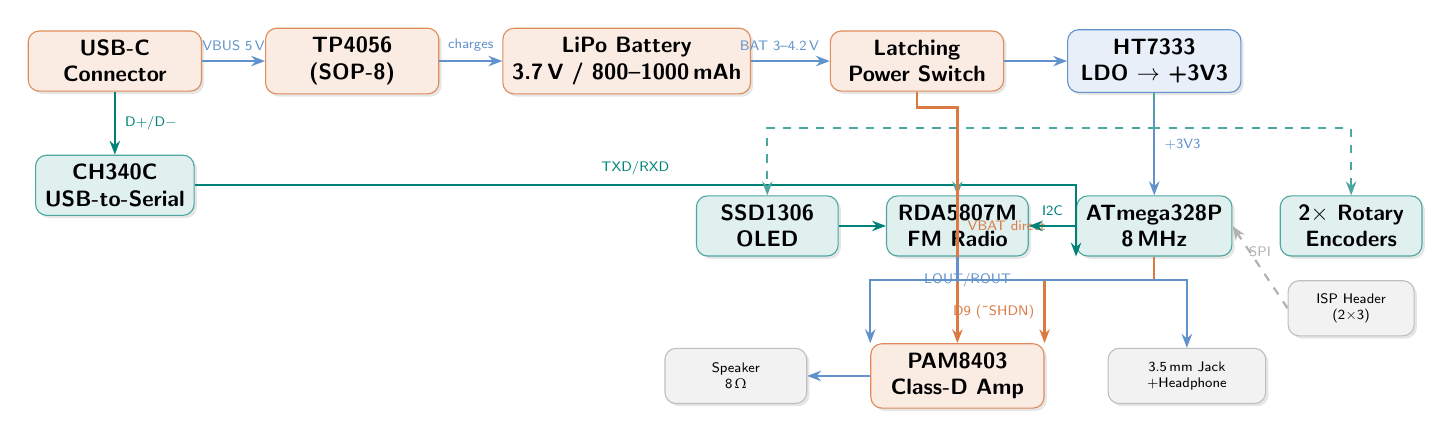
\begin{tikzpicture}[
  box/.style={draw=accentblue!70, fill=accentblue!10, rounded corners=4pt,
              minimum width=2.2cm, minimum height=0.7cm,
              font=\sffamily\footnotesize\bfseries, align=center,
              drop shadow={shadow xshift=1pt,shadow yshift=-1pt,opacity=0.2}},
  sbox/.style={box, fill=accentteal!12, draw=accentteal!70},
  pbox/.style={box, fill=accentorange!12, draw=accentorange!70},
  gbox/.style={box, fill=gray!10, draw=gray!50, font=\sffamily\tiny},
  arr/.style={-{Stealth[length=5pt]}, thick, color=accentblue!70},
  label/.style={font=\sffamily\tiny\color{codegray}},
  node distance=0.5cm and 0.8cm
]

% Power / charging
\node[pbox, minimum width=2.2cm] (usbc) {USB-C\\Connector};
\node[pbox, right=0.8cm of usbc, minimum width=2.2cm] (tp4056) {TP4056\\(SOP-8)};
\node[pbox, right=0.8cm of tp4056, minimum width=2.8cm] (lipo) {LiPo Battery\\3.7\,V / 800--1000\,mAh};
\node[pbox, right=1.0cm of lipo, minimum width=2.2cm] (sw) {Latching\\Power Switch};
\node[box, right=0.8cm of sw, minimum width=2.2cm] (ldo) {HT7333\\LDO $\rightarrow$ +3V3};

% USB-C also goes to CH340C
\node[sbox, below=0.8cm of usbc, minimum width=2.0cm] (ch340) {CH340C\\USB-to-Serial};

% 3V3 consumers
\node[sbox, below=1.3cm of ldo, minimum width=1.8cm] (mcu) {ATmega328P\\8\,MHz};
\node[sbox, left=0.6cm of mcu, minimum width=1.8cm] (radio) {RDA5807M\\FM Radio};
\node[sbox, left=0.6cm of radio, minimum width=1.8cm] (oled) {SSD1306\\OLED};
\node[sbox, right=0.6cm of mcu, minimum width=1.8cm] (enc) {2$\times$ Rotary\\Encoders};

% Audio / output
\node[pbox, below=1.1cm of radio, minimum width=2.2cm] (amp) {PAM8403\\Class-D Amp};
\node[gbox, left=0.8cm of amp, minimum width=1.8cm] (spk) {Speaker\\8\,$\Omega$};
\node[gbox, right=0.8cm of amp, minimum width=2.0cm] (jack) {3.5\,mm Jack\\+Headphone};

% Arrows --- power chain
\draw[arr] (usbc) -- node[label,above]{VBUS 5\,V} (tp4056);
\draw[arr] (tp4056) -- node[label,above]{charges} (lipo);
\draw[arr] (lipo) -- node[label,above,xshift=-4pt]{BAT 3--4.2\,V} (sw);
\draw[arr] (sw) -- (ldo);
\draw[arr] (ldo) -- node[label,right]{+3V3} (mcu);

% USB-C to CH340C
\draw[arr,color=accentteal] (usbc.south) -- node[label,right]{D+/D$-$} (ch340.north);
\draw[arr,color=accentteal] (ch340.east) -| node[label,near start,above]{TXD/RXD} (mcu.south west);

% 3V3 rail distribution (dashed)
\draw[arr,dashed,color=accentteal!70] (ldo.south) -- ++(0,-0.45) -| (radio.north);
\draw[arr,dashed,color=accentteal!70] (ldo.south) -- ++(0,-0.45) -| (oled.north);
\draw[arr,dashed,color=accentteal!70] (ldo.south) -- ++(0,-0.45) -| (enc.north);

% VBAT to amp (direct)
\draw[arr,color=accentorange!80] (sw.south) -- ++(0,-0.2) -| node[label,near end,right]{VBAT direct} (amp.north);

% I2C
\draw[arr, color=accentteal] (mcu) -- node[label,above]{I2C} (radio);
\draw[arr, color=accentteal] (oled) -- (radio);

% MCU → amp SHDN
\draw[arr, color=accentorange!80] (mcu.south) -- ++(0,-0.3) -| node[label,near end,left]{D9 (\textasciitilde{}SHDN)} (amp.north east);

% Audio
\draw[arr] (radio.south) -- ++(0,-0.3) -| node[label,near start,right]{LOUT/ROUT} (amp.north west);
\draw[arr] (amp) -- (spk);
\draw[arr] (radio.south) -- ++(0,-0.3) -| (jack.north);

% ISP header (small)
\node[gbox, below=0.3cm of enc, minimum width=1.6cm] (isp) {ISP Header\\(2$\times$3)};
\draw[arr,dashed,color=gray!60] (isp.west) -- node[label,above]{SPI} (mcu.east);

\end{tikzpicture}
\end{diagrambox}

\subsection{Power Architecture}

\begin{infobox}
The ATmega328P runs at \textbf{3.3\,V and 8\,MHz}. This is within the official specification (datasheet: 2.4--5.5\,V for $\leq$10\,MHz). Running at 3.3\,V means:
\begin{itemize}[noitemsep]
    \item \textbf{No level shifters needed} --- MCU, radio, and OLED all share the same 3.3\,V rail
    \item \textbf{Lower power consumption} --- longer battery life
    \item \textbf{Use an 8\,MHz crystal} (not 16\,MHz)
    \item Bootloader: ``Arduino Pro Mini 3.3\,V 8\,MHz'' in Arduino IDE
\end{itemize}
\end{infobox}

\begin{itemize}[noitemsep]
    \item \textbf{USB-C VBUS (5\,V)} $\rightarrow$ TP4056 IN+ $\rightarrow$ charges LiPo (4.2\,V CC/CV)
    \item \textbf{USB-C D+/D$-$} $\rightarrow$ CH340C $\rightarrow$ ATmega UART (firmware upload)
    \item \textbf{LiPo BAT+} $\rightarrow$ TP4056 BAT (pin 3) $\rightarrow$ latching switch $\rightarrow$ \textbf{VBAT} bus (3.0--4.2\,V)
    \item \textbf{LiPo BAT$-$} $\rightarrow$ DW01A/FS8205A protection (low-side, on BAT$-$ path) $\rightarrow$ GND bus. The DW01A monitors cell voltage; the FS8205A dual N-FET pair sits between BAT$-$ and circuit GND, disconnecting the ground return on over-discharge, over-charge, or short-circuit.
    \item \textbf{VBAT} $\rightarrow$ HT7333 LDO ($<$100\,mV dropout) $\rightarrow$ \textbf{+3V3} rail (MCU + radio + OLED + encoders + CH340C)
    \item \textbf{VBAT} $\rightarrow$ PAM8403 VDD directly (no LDO --- maximises audio power; PAM8403 accepts 2.5--5.5\,V)
    \item \textbf{VBAT} $\rightarrow$ 100\,k / 100\,k voltage divider $\rightarrow$ ATmega A0 (battery sensing)
\end{itemize}

\begin{warningbox}
The HT7333 LDO has $<$100\,mV dropout. At battery minimum (3.0\,V), output is $\sim$2.9\,V. The ATmega328P runs reliably at 2.9\,V / 8\,MHz (min spec 2.4\,V). \\
\textbf{Do NOT use AMS1117-3.3} --- it requires 1\,V headroom and will fail below 4.3\,V battery.
\end{warningbox}

\subsection{DW01A + FS8205A Battery Protection (Low-Side)}

The DW01A + FS8205A form a \textbf{low-side} battery protection circuit on the BAT$-$ path. The FS8205A contains two N-channel MOSFETs in a single SOT-23-6 package. Because they are N-FETs, they \textbf{must} sit on the low side (between BAT$-$ and circuit GND), not on BAT+.

\begin{diagrambox}
\centering
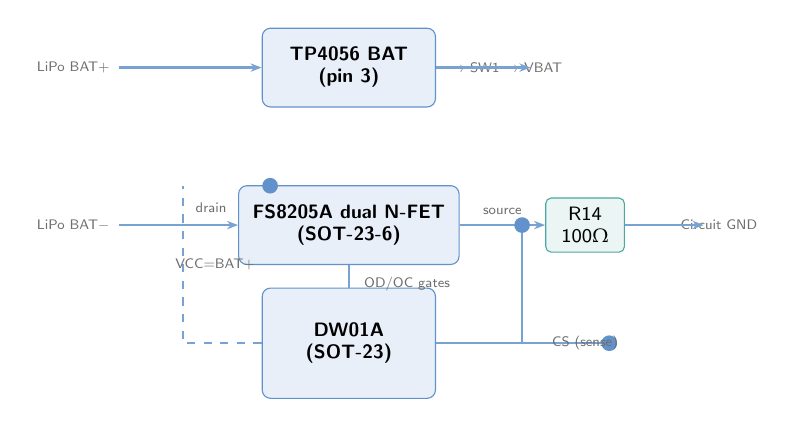
\begin{tikzpicture}[
  ic/.style={draw=accentblue!70, fill=accentblue!10, rounded corners=3pt,
             minimum width=2.2cm, minimum height=1.0cm,
             font=\sffamily\scriptsize\bfseries, align=center},
  comp/.style={draw=accentteal!70, fill=accentteal!8, rounded corners=2pt,
               minimum width=1.0cm, minimum height=0.45cm,
               font=\sffamily\scriptsize, align=center},
  arr/.style={-{Stealth[length=4pt]}, thick, color=accentblue!60},
  wire/.style={thick, color=accentblue!60},
  lbl/.style={font=\sffamily\tiny, color=codegray, align=left},
  dot/.style={fill=accentblue!70, circle, inner sep=2pt}
]
% Battery
\node[lbl] (batp) at (0,2) {LiPo BAT+};
\node[lbl] (batn) at (0,0) {LiPo BAT$-$};

% TP4056 / Load path
\node[ic] (tp) at (3.5,2) {TP4056 BAT\\(pin 3)};
\draw[arr] (batp.east) -- (tp.west);
\node[lbl] at (5.5,2) {$\to$ SW1 $\to$ VBAT};
\draw[arr] (tp.east) -- ++(1.2,0);

% DW01A
\node[ic, minimum height=1.4cm] (dw) at (3.5,-1.5) {DW01A\\(SOT-23)};

% FS8205A
\node[ic, minimum width=2.8cm, minimum height=1.0cm] (fs) at (3.5,0) {FS8205A dual N-FET\\(SOT-23-6)};

% R14 sense resistor
\node[comp] (r14) at (6.5,0) {R14\\100$\Omega$};
\node[lbl] at (8.2,0) {Circuit GND};
\draw[arr] (r14.east) -- ++(1.0,0);

% BAT- to FS8205A drain
\draw[arr] (batn.east) -- (fs.west);
\node[lbl, above=1pt] at (1.75,0) {drain};

% FS8205A source to R14
\draw[arr] (fs.east) -- node[lbl,above]{source} (r14.west);

% DW01A connections
\draw[wire] (dw.north) -- (fs.south);
\node[lbl, right=2pt] at (3.5,-0.75) {OD/OC gates};
\draw[wire] (dw.east) -- ++(2.2,0) -- ++(0,0.0) node[dot]{};
\node[lbl] at (6.5,-1.5) {CS (sense)};
% CS connects to R14/FS8205A junction
\draw[wire] (5.7,-1.5) -- (5.7,0);
\node[dot] at (5.7,0) {};

% DW01A VCC = BAT+
\draw[wire,dashed] (dw.west) -- ++(-1.0,0) -- ++(0,2.0);
\node[dot] at (2.5,0.5) {};
\node[lbl, left=2pt] at (2.5,-0.5) {VCC=BAT+};

\end{tikzpicture}
\end{diagrambox}

\begin{infobox}
\textbf{DW01A + FS8205A wiring summary:}
\begin{itemize}[noitemsep]
  \item \textbf{DW01A VCC} $\leftarrow$ LiPo BAT+ (monitors cell voltage directly)
  \item \textbf{DW01A GND} $\rightarrow$ FS8205A source / R14 junction
  \item \textbf{DW01A OD} (over-discharge gate) $\rightarrow$ FS8205A gate 1
  \item \textbf{DW01A OC} (over-charge gate) $\rightarrow$ FS8205A gate 2
  \item \textbf{DW01A CS} (current sense) $\leftarrow$ R14/FS8205A source junction
  \item \textbf{FS8205A drain} $\leftarrow$ LiPo BAT$-$
  \item \textbf{FS8205A source} $\rightarrow$ R14 (100\,$\Omega$) $\rightarrow$ circuit GND bus
  \item \textbf{R14} senses over-current conditions (short-circuit protection)
\end{itemize}
\end{infobox}

\subsection{Audio Signal Path}

\begin{diagrambox}
\centering
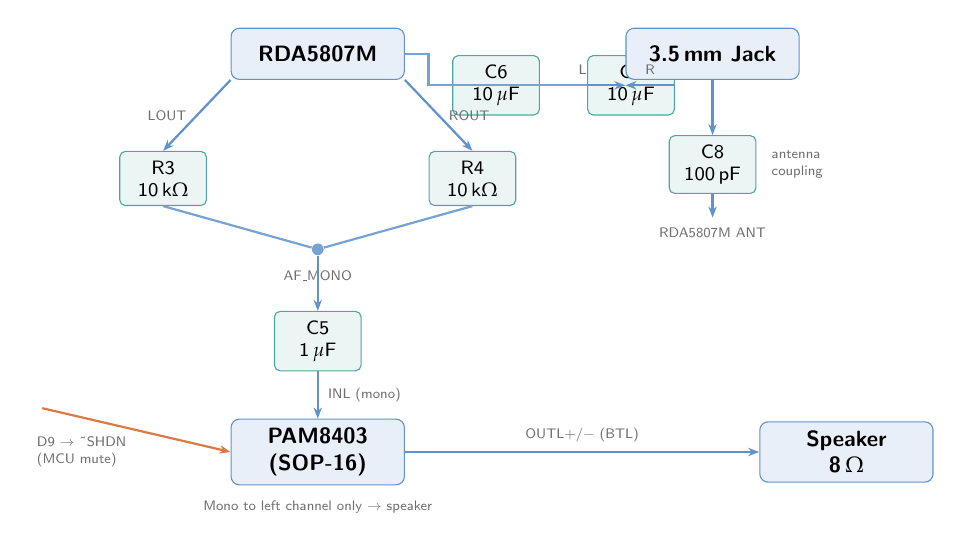
\begin{tikzpicture}[
  ic/.style={draw=accentblue!70, fill=accentblue!10, rounded corners=3pt,
             minimum width=2.2cm, minimum height=0.65cm,
             font=\sffamily\footnotesize\bfseries, align=center},
  comp/.style={draw=accentteal!70, fill=accentteal!8, rounded corners=2pt,
               minimum width=1.1cm, minimum height=0.55cm,
               font=\sffamily\scriptsize, align=center},
  node/.style={circle, fill=accentblue!60, inner sep=1.5pt},
  wire/.style={thick, color=accentblue!60},
  label/.style={font=\sffamily\tiny, color=codegray, align=left},
  arr/.style={-{Stealth[length=4pt]}, thick, color=accentblue!70}
]
% --- Nodes ---
\node[ic] (rda) {RDA5807M};
\node[comp, below left=0.9cm and 0.3cm of rda] (r3) {R3\\10\,k$\Omega$};
\node[comp, below right=0.9cm and 0.3cm of rda] (r4) {R4\\10\,k$\Omega$};
\node[node] (mix) at ($(r3)!0.5!(r4) + (0,-0.9cm)$) {};
\node[label, below=2pt of mix] {AF\_MONO};
\node[comp, below=0.7cm of mix] (c5) {C5\\1\,$\mu$F};
\node[ic, below=0.6cm of c5] (pam) {PAM8403\\(SOP-16)};
\node[ic, right=4.5cm of pam] (spk) {Speaker\\8\,$\Omega$};
\node[comp, right=0.6cm of rda, yshift=-0.4cm] (c6) {C6\\10\,$\mu$F};
\node[comp, right=0.6cm of c6] (c7) {C7\\10\,$\mu$F};
\node[ic, right=2.8cm of rda] (jack) {3.5\,mm Jack};
\node[comp, below=0.7cm of jack] (c8) {C8\\100\,pF};

% --- MCU SHDN control ---
\node[label, left=1.2cm of pam] {D9 $\to$ \textasciitilde{}SHDN\\(MCU mute)};
\draw[arr, color=accentorange!80] (-3.5,-4.5) -- (pam.west);

% --- Wires ---
\draw[arr] (rda.south west) -- node[label,left]{LOUT} (r3.north);
\draw[arr] (rda.south east) -- node[label,right]{ROUT} (r4.north);
\draw[wire] (r3.south) -- (mix);
\draw[wire] (r4.south) -- (mix);
\draw[arr] (mix) -- (c5);
\draw[arr] (c5) -- node[label,right]{INL (mono)} (pam.north);
\draw[arr] (pam.east) -- node[label,above]{OUTL+/$-$ (BTL)} (spk.west);
\node[label, below=2pt of pam] {Mono to left channel only $\to$ speaker};

% Headphone path
\draw[wire] (rda.east) -- ++(0.3,0) |- (c6.west);
\draw[arr] (c6.east) -- node[label,above]{L} (jack.west|-c6);
\draw[wire] (rda.east) -- ++(0.3,0) |- (c7.west);
\draw[arr] (c7.east) -- node[label,above]{R} (jack.west|-c7);

% Antenna coupling
\draw[arr] (jack.south) -- (c8.north);
\draw[arr] (c8.south) -- ++(0,-0.3) node[label,below]{RDA5807M ANT};
\node[label, right=2pt of c8] {antenna\\coupling};

\end{tikzpicture}
\end{diagrambox}

Volume is controlled digitally via RDA5807M register 0x05 bits [3:0], range 0--15, adjusted by the left rotary encoder. No hardware potentiometer.

\begin{infobox}
\textbf{Audio topology --- mono speaker, stereo headphones:} The RDA5807M outputs stereo on LOUT/ROUT. For the \textbf{speaker path}, R3 and R4 (each 10\,k$\Omega$) passively sum LOUT + ROUT into a single mono signal (AF\_MONO). This feeds through a single coupling capacitor C5 (1\,$\mu$F) into PAM8403 \textbf{INL (pin 8) only}. INR (pin 7) is tied to GND via a 10\,k$\Omega$ resistor to prevent noise pickup. Only the left BTL channel (OUTL+/OUTL$-$) drives the speaker. For the \textbf{headphone path}, LOUT and ROUT connect directly (via C6 and C7) to the 3.5\,mm jack TIP and RING, preserving full stereo.
\end{infobox}

When headphones are plugged in, the MCU detects the insertion via D8 (HP\_DETECT, jack pin 2) and pulls D9 LOW, which drives the PAM8403 \textasciitilde{}SHDN pin LOW to mute the amplifier. Audio is routed to headphones via the coupling capacitors C6/C7. When headphones are removed, D9 goes HIGH and the speaker resumes.

% ============================================================================
\section{Complete Bill of Materials}
% ============================================================================

\subsection{ICs and Modules}

\begin{longtable}{@{}p{1cm}p{4cm}p{1.5cm}p{1cm}p{5cm}@{}}
\toprule
\textbf{Ref} & \textbf{Part} & \textbf{Package} & \textbf{Qty} & \textbf{Notes} \\
\midrule
\endhead
U1 & ATmega328P-PU & DIP-28 & 1 & Main MCU. Through-hole. Same as Arduino UNO chip. \\
U2 & RDA5807M (RRD-102 V2.0) & Module & 1 & \textbf{Already owned.} Solders onto 2$\times$5 pin header pads. \\
U3 & \textbf{PAM8403} & SOP-16 & 1 & Class-D amplifier. Wired mono (left channel only to 8\,$\Omega$ speaker). $\sim$0.5\,W at 3.7\,V into 8\,$\Omega$. \textasciitilde{}SHDN pin for MCU mute. \textbf{SMD --- workshop solders.} \\
U4 & \textbf{TP4056} & SOP-8 & 1 & LiPo CC/CV charger IC. On main PCB sharing USB-C VBUS. \textbf{SMD --- workshop solders.} \\
U5 & \textbf{HT7333} & SOT-89 & 1 & 3.3\,V LDO regulator, 250\,mA, low dropout ($<$100\,mV). \textbf{SMD --- workshop solders.} \\
U6 & \textbf{CH340C} & SOP-16 & 1 & USB-to-serial bridge. Connects USB-C D+/D- to ATmega UART. No external crystal needed. \textbf{SMD --- workshop solders.} \\
U7 & DW01A + FS8205A & SOT-23 + SOT-23-6 & 1+1 & Battery protection: over-discharge, over-charge, short-circuit. \textbf{SMD --- workshop solders.} \\
--- & SSD1306 0.96'' OLED & Module & 1 & \textbf{Already owned.} 4-pin I2C. Plugs into header. \\
\bottomrule
\end{longtable}

\subsection{Resistors}

\begin{longtable}{@{}p{1cm}p{2cm}p{1cm}p{8.5cm}@{}}
\toprule
\textbf{Ref} & \textbf{Value} & \textbf{Qty} & \textbf{Purpose} \\
\midrule
\endhead
R1 & 4.7\,k$\Omega$ & 1 & I2C SDA pull-up to +3V3 \\
R2 & 4.7\,k$\Omega$ & 1 & I2C SCL pull-up to +3V3 \\
R3 & 10\,k$\Omega$ & 1 & RDA5807M LOUT $\rightarrow$ mono mix resistor (summed with R4 to AF\_MONO) \\
R4 & 10\,k$\Omega$ & 1 & RDA5807M ROUT $\rightarrow$ mono mix resistor (summed with R3 to AF\_MONO) \\
R5 & 10\,k$\Omega$ & 1 & ATmega RESET pull-up to +3V3 \\
R6 & 330\,$\Omega$ & 1 & Power LED current limiter (from +3V3) \\
R7 & 100\,k$\Omega$ & 1 & Battery divider --- top (VBAT to ADC) \\
R8 & 100\,k$\Omega$ & 1 & Battery divider --- bottom (ADC to GND) \\
R9 & 2.2\,k$\Omega$ & 1 & TP4056 PROG pin --- sets charge current to $\sim$455\,mA ($I_{charge} = 1000/R9$). For 800\,mAh cell: $\sim$0.57C. Charges in $\sim$2\,hrs. Use 10\,k$\Omega$ for 100\,mA (very slow), 1.2\,k$\Omega$ for 1\,A (check USB source). \\
R10 & 5.1\,k$\Omega$ & 1 & USB-C CC1 pull-down (tells charger ``I am a device'') \\
R11 & 5.1\,k$\Omega$ & 1 & USB-C CC2 pull-down \\
R12 & 1\,k$\Omega$ & 1 & CHG LED current limiter: VBUS $\to$ R12 $\to$ LED2 $\to$ TP4056 CHRG pin 7 (open-drain) \\
R13 & 1\,k$\Omega$ & 1 & STDBY LED current limiter: VBUS $\to$ R13 $\to$ LED3 $\to$ TP4056 STDBY pin 6 (open-drain) \\
R14 & 100\,$\Omega$ & 1 & DW01A current sense resistor between FS8205A source pins and circuit GND (low-side topology) \\
\bottomrule
\end{longtable}

\subsection{Capacitors}

\begin{longtable}{@{}p{1cm}p{2cm}p{2cm}p{1cm}p{6cm}@{}}
\toprule
\textbf{Ref} & \textbf{Value} & \textbf{Type} & \textbf{Qty} & \textbf{Purpose} \\
\midrule
\endhead
C1 & 100\,nF & Ceramic & 1 & ATmega VCC decoupling \\
C2 & 100\,nF & Ceramic & 1 & ATmega AVCC decoupling \\
C3 & 22\,pF & Ceramic & 2 & Crystal load capacitors (8\,MHz) \\
C4 & 100\,nF & Ceramic & 1 & RDA5807M VCC decoupling \\
C5 & 1\,$\mu$F & Ceramic & 1 & PAM8403 input coupling (mono-mixed AF\_MONO $\to$ INL only) \\
C6 & 10\,$\mu$F & Electrolytic & 1 & Headphone L coupling (LOUT to jack TIP) \\
C7 & 10\,$\mu$F & Electrolytic & 1 & Headphone R coupling (ROUT to jack RING) \\
C8 & 100\,pF & Ceramic & 1 & Antenna coupling (jack TIP to RDA ANT pin) \\
C9 & 10\,$\mu$F & Electrolytic & 1 & HT7333 LDO input bypass \\
C10 & 10\,$\mu$F & Electrolytic & 1 & HT7333 LDO output bypass \\
C11 & 10\,$\mu$F & Ceramic & 1 & PAM8403 PVCC bypass \\
C12 & 10\,$\mu$F & Ceramic & 1 & TP4056 input bypass (USB-C VBUS) \\
C13 & 100\,nF & Ceramic & 1 & CH340C VCC decoupling \\
C14 & 100\,nF & Ceramic & 1 & Auto-reset cap (CH340C DTR\# $\to$ ATmega RESET) \\
C15 & 1\,$\mu$F & Ceramic & 1 & TP4056 output bypass \\
C16 & 10\,$\mu$F & Electrolytic & 1 & RDA5807M VCC bulk \\
C17 & 1\,$\mu$F & Ceramic & 1 & TP4056 BAT pin decoupling \\
C18 & 100\,nF & Ceramic & 1 & CH340C V3 pin (pin 4) bypass --- required for USB enumeration \\
C19 & 100\,nF & Ceramic & 1 & ADC filter: A0 divider midpoint to GND. Reduces source impedance for ATmega328P ADC (100\,k$\Omega$\;||\;100\,k$\Omega$ = 50\,k$\Omega$ too high without cap). \\
C20 & 10\,$\mu$F & Ceramic & 1 & PAM8403 PVCC pin 15 bypass (each PVCC pin needs its own bypass cap) \\
C21 & 100\,nF & Ceramic & 1 & ATmega AREF pin to GND --- stabilises ADC reference voltage \\
\bottomrule
\end{longtable}

\subsection{Connectors, Switches, and Mechanical}

\begin{longtable}{@{}p{1cm}p{4.5cm}p{1cm}p{6cm}@{}}
\toprule
\textbf{Ref} & \textbf{Part} & \textbf{Qty} & \textbf{Notes} \\
\midrule
\endhead
J1 & 3.5\,mm TRS audio jack with detect pin & 1 & PJ-320A \textbf{NO-type} (Normally Open detect). When no plug is inserted, the detect pin floats; when a plug is inserted, the detect pin connects to sleeve (GND). This is the variant with a \textbf{5th pin} for detection. Do \textbf{not} use the NC (Normally Closed) variant. \\
J2 & JST PH 2-pin connector & 1 & LiPo battery connector \\
J3 & 2$\times$3 pin header (2.54\,mm) & 1 & AVR ISP programming header --- bootloader burn (one-time) \\
J4 & USB-C receptacle (SMD, 16-pin) & 1 & \textbf{Both charging and programming.} Use GCT USB4105 or equivalent \textbf{16-pin} SMD receptacle. D+ / D- to CH340C; VBUS to TP4056. \textbf{Workshop solders.} \\
J5 & 1$\times$4 pin header (2.54\,mm) & 1 & OLED module connector (GND, VCC, SCL, SDA) \\
J6 & 1$\times$5 pin header (2.54\,mm) & 2 & Encoder connectors \\
J7 & 2$\times$5 pin header (1.27\,mm pitch) & 1 & RRD-102 radio module pads (castellated edge, 1.27\,mm) \\
J8 & 1$\times$2 pad or connector & 1 & Speaker output \\
J9 & Solder pad & 1 & Backup wire antenna \\
--- & Right encoder + knob cap & 1 & Tuning. \\
--- & Left encoder + knob cap & 1 & Volume. \\
SW1 & Latching push button & 1 & Power ON/OFF \\
LED1 & Red 3\,mm LED & 1 & Power indicator (from +3V3) \\
LED2 & Red SMD LED (0805) & 1 & TP4056 CHG indicator (charging) \\
LED3 & Green SMD LED (0805) & 1 & TP4056 STDBY indicator (full) \\
Y1 & 8\,MHz crystal (HC49S) & 1 & ATmega clock source \\
SPK1 & 8\,$\Omega$ 0.5--1\,W speaker (28--40\,mm) & 1 & Built-in speaker \\
BAT1 & LiPo 3.7\,V 800--1000\,mAh flat & 1 & With JST PH connector \\
\bottomrule
\end{longtable}

\subsection{Mechanical (Enclosure)}

\begin{longtable}{@{}p{5cm}p{1cm}p{6.5cm}@{}}
\toprule
\textbf{Part} & \textbf{Qty} & \textbf{Notes} \\
\midrule
\endhead
Clear acrylic sheet 2--3\,mm & 1 & For laser cutting enclosure layers \\
M3$\times$20\,mm bolts & 4 & Corner bolts \\
M3 nuts & 4 & To hold bolts \\
M3$\times$5\,mm nylon standoffs & 4 & PCB mounting \\
Rubber feet (adhesive) & 4 & Optional, for bottom \\
\bottomrule
\end{longtable}

\subsection{Estimated Cost}

\begin{longtable}{@{}p{6cm}p{3cm}@{}}
\toprule
\textbf{Item} & \textbf{Approx (Rs.)} \\
\midrule
\endhead
ATmega328P-PU & 300--500 \\
PAM8403 Class-D amplifier (SOP-16) & 80--150 \\
CH340C USB-to-serial (SOP-16) & 80--150 \\
TP4056 charger IC (SOP-8) & 30--60 \\
HT7333 LDO (SOT-89) & 30--60 \\
DW01A + FS8205A battery protection & 30--50 \\
USB-C receptacle (SMD) & 80--150 \\
Crystal + caps + resistors + LEDs & 150--300 \\
3.5\,mm audio jack & 30--60 \\
Small speaker (8\,$\Omega$) & 100--200 \\
LiPo 800--1000\,mAh & 400--800 \\
2$\times$ encoders + knob caps & 200--400 \\
Latching push button & 30--50 \\
PCB fabrication (2-layer, 5 pcs, $\sim$70$\times$50\,mm) & 800--1500 \\
Acrylic cutting & 200--500 \\
M3 hardware & 100--200 \\
\midrule
\textbf{Total} & \textbf{Rs.\,2650--5130} \\
\bottomrule
\end{longtable}

% ============================================================================
\section{Complete Circuit Design}
\label{sec:circuit}
% ============================================================================

\begin{dangerbox}
\begin{enumerate}[noitemsep]
    \item \textbf{RDA5807M is a 3.3\,V device.} Never connect 5\,V to VCC. Instant destruction.
    \item \textbf{I2C pull-ups go to +3V3 only.} Never to 5\,V or VBAT.
    \item \textbf{LiPo battery safety:} Never short-circuit. Never charge unattended. Never puncture.
    \item \textbf{TP4056 PROG resistor (R9):} Sets charge current ($I = 1000/R9$). 2.2\,k$\Omega$ = 455\,mA, 10\,k$\Omega$ = 100\,mA, 1.2\,k$\Omega$ = 1\,A. Match to battery capacity.
    \item \textbf{PAM8403 outputs are BTL:} Neither speaker wire goes to GND. Bridging either to GND will damage the IC.
    \item \textbf{USB-C data lines:} D+ and D$-$ go to CH340C only. Do not short VBUS to D+/D$-$.
    \item \textbf{Electrolytic capacitor polarity matters.} Reversed = burst/fire.
\end{enumerate}
\end{dangerbox}

\subsection{ATmega328P Pin Assignment}

\begin{longtable}{@{}p{1.5cm}p{2.5cm}p{2.5cm}p{6cm}@{}}
\toprule
\textbf{ATmega Pin} & \textbf{Arduino Pin} & \textbf{Net Name} & \textbf{Function} \\
\midrule
\endhead
1 (PC6) & RESET & RESET & 10\,k$\Omega$ pull-up to +3V3 + ISP pin 5 + CH340C DTR\# via C14 (100\,nF auto-reset) \\
2 (PD0) & D0 (RX) & UART\_RX & CH340C TXD --- receives data from USB-C \\
3 (PD1) & D1 (TX) & UART\_TX & CH340C RXD --- transmits data to USB-C \\
4 (PD2) & D2 (INT0) & ENC\_R\_CLK & Right encoder CLK --- hardware interrupt \\
5 (PD3) & D3 (INT1) & ENC\_L\_CLK & Left encoder CLK --- hardware interrupt \\
6 (PD4) & D4 & ENC\_R\_DT & Right encoder DT \\
7 (VCC) & VCC & +3V3 & Power + C1 (100\,nF) to GND \\
8 (GND) & GND & GND & Digital ground \\
9 (PB6) & XTAL1 & XTAL1 & 8\,MHz crystal + C3a (22\,pF) to GND \\
10 (PB7) & XTAL2 & XTAL2 & 8\,MHz crystal + C3b (22\,pF) to GND \\
11 (PD5) & D5 & ENC\_L\_DT & Left encoder DT \\
12 (PD6) & D6 & ENC\_R\_SW & Right encoder button (press = Seek UP) \\
13 (PD7) & D7 & ENC\_L\_SW & Left encoder button (press = Seek DOWN) \\
14 (PB0) & D8 & HP\_DETECT & 3.5\,mm jack detect (LOW = plugged in) \\
15 (PB1) & D9 & AMP\_EN & PAM8403 \textasciitilde{}SHDN pin. HIGH = amplifier on, LOW = mute. MCU-controlled speaker muting when HP detected on D8. \\
16 (PB2) & D10 & --- & Unused (available) \\
17 (PB3) & D11 (MOSI) & ISP\_MOSI & ISP header pin 4 \\
18 (PB4) & D12 (MISO) & ISP\_MISO & ISP header pin 1 \\
19 (PB5) & D13 (SCK) & ISP\_SCK & ISP header pin 3 \\
20 (AVCC) & AVCC & +3V3 & Analog power + C2 (100\,nF) to GND \\
21 (AREF) & AREF & --- & C21 (100\,nF) to GND for ADC reference stability. Leave electrically floating (internal AREF). \\
22 (GND) & AGND & GND & Analog ground \\
23 (PC0) & A0 & BAT\_SENSE & Voltage divider midpoint (VBAT/2) \\
24 (PC1) & A1 & --- & Unused \\
25 (PC2) & A2 & --- & Unused \\
26 (PC3) & A3 & --- & Unused \\
27 (PC4) & A4 (SDA) & I2C\_SDA & I2C data: RDA5807M + SSD1306 \\
28 (PC5) & A5 (SCL) & I2C\_SCL & I2C clock: RDA5807M + SSD1306 \\
\bottomrule
\end{longtable}

\textbf{Total GPIOs used: 13 of 23 available. Plenty of headroom for future features.}

\subsection{TP4056 LiPo Charger IC (SOP-8, On-Board)}

The TP4056 is a \textbf{surface-mount CC/CV LiPo charger IC} (SOP-8) soldered directly onto the main PCB by the university workshop. It shares the USB-C VBUS line for 5\,V input. Battery protection is provided by a separate DW01A + FS8205A pair.

\begin{diagrambox}
\centering
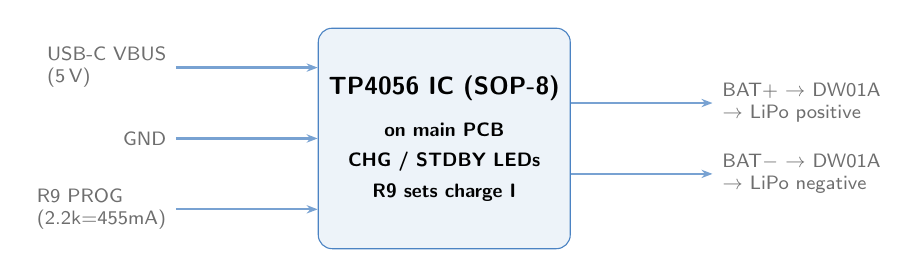
\begin{tikzpicture}[
  mod/.style={draw=accentblue!80, fill=accentblue!8, rounded corners=5pt,
              minimum width=3.2cm, minimum height=2.8cm,
              font=\sffamily\small\bfseries, align=center},
  lbl/.style={font=\sffamily\scriptsize, color=codegray, align=left},
  arr/.style={-{Stealth[length=4pt]}, thick, color=accentblue!60},
  node distance=0.6cm]
\node[mod] (mod) {TP4056 IC (SOP-8)\\[4pt]{\scriptsize on main PCB}\\{\scriptsize CHG / STDBY LEDs}\\{\scriptsize R9 sets charge I}};

\node[lbl, left=1.8cm of mod, yshift= 0.9cm] (vin)  {USB-C VBUS\\(5\,V)};
\node[lbl, left=1.8cm of mod, yshift= 0.0cm] (gnd)  {GND};
\node[lbl, left=1.8cm of mod, yshift=-0.9cm] (prog) {R9 PROG\\(2.2k=455mA)};
\node[lbl, right=1.8cm of mod, yshift= 0.45cm] (bp)  {BAT+ $\to$ DW01A\\$\to$ LiPo positive};
\node[lbl, right=1.8cm of mod, yshift=-0.45cm] (bm)  {BAT$-$ $\to$ DW01A\\$\to$ LiPo negative};

\draw[arr] (vin.east)   -- (mod.west|-vin);
\draw[arr] (gnd.east)   -- (mod.west|-gnd);
\draw[arr] (prog.east)  -- (mod.west|-prog);
\draw[arr] (mod.east|-bp) -- (bp.west);
\draw[arr] (mod.east|-bm) -- (bm.west);
\end{tikzpicture}
\end{diagrambox}

\begin{infobox}
\textbf{TP4056 IC on-board connections:}
\begin{itemize}[noitemsep]
  \item \textbf{VCC (pin 4)} $\leftarrow$ USB-C VBUS (5\,V) + C12 (10\,$\mu$F) bypass
  \item \textbf{PROG (pin 2)} $\rightarrow$ R9 to GND. 2.2\,k$\Omega$ = $\sim$455\,mA charge current (safe for 800\,mAh cell, charges in $\sim$2\,hrs). Use 10\,k$\Omega$ for 100\,mA (slow/safe), 1.2\,k$\Omega$ for $\sim$1\,A.
  \item \textbf{BAT (pin 3)} $\rightarrow$ DW01A/FS8205A $\rightarrow$ LiPo battery via JST J2. Plus C17 (1\,$\mu$F) bypass.
  \item \textbf{CHRG (pin 7)} $\leftarrow$ open-drain sink. Wire: USB VBUS $\rightarrow$ R12 (1\,k$\Omega$) $\rightarrow$ LED2 (red, anode to R12) $\rightarrow$ CHRG pin 7. The IC sinks current through the LED when charging.
  \item \textbf{STDBY (pin 6)} $\leftarrow$ open-drain sink. Wire: USB VBUS $\rightarrow$ R13 (1\,k$\Omega$) $\rightarrow$ LED3 (green, anode to R13) $\rightarrow$ STDBY pin 6. The IC sinks current through the LED when battery is full.
  \item \textbf{GND (pin 1, 5)} $\rightarrow$ GND plane.
  \item \textbf{CE (pin 8)} $\rightarrow$ VCC (always enabled).
\end{itemize}
\end{infobox}

\begin{warningbox}
\textbf{Never place the power switch between the battery and BAT+!} The DW01A protection circuit needs a permanent battery connection to monitor cell voltage. The latching power switch must be on the \textbf{VBAT line} (after DW01A output), not between battery and TP4056.
\end{warningbox}

\subsection{Power Switch and LDO}

\begin{diagrambox}
\centering
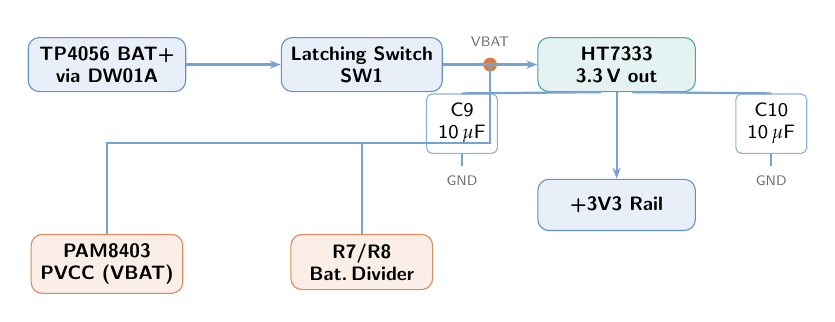
\begin{tikzpicture}[
  box/.style={draw=accentblue!70, fill=accentblue!10, rounded corners=4pt,
              minimum width=2.0cm, minimum height=0.65cm,
              font=\sffamily\scriptsize\bfseries, align=center},
  sbox/.style={box, fill=accentteal!10, draw=accentteal!70},
  comp/.style={draw=accentblue!50, fill=white, rounded corners=2pt,
               minimum width=0.9cm, minimum height=0.45cm,
               font=\sffamily\scriptsize, align=center},
  arr/.style={-{Stealth[length=4pt]}, thick, color=accentblue!60},
  wire/.style={thick, color=accentblue!60},
  lbl/.style={font=\sffamily\tiny, color=codegray},
  gnd/.style={lbl},
  node distance=0.5cm and 1.0cm
]
\node[box] (bat) {TP4056 BAT+\\via DW01A};
\node[box, right=1.2cm of bat] (sw) {Latching Switch\\SW1};
\node[sbox, right=1.2cm of sw] (ldo) {HT7333\\3.3\,V out};
\node[box, below=1.1cm of ldo] (rail) {+3V3 Rail};
\node[comp, left=0.5cm of ldo.south west, yshift=-0.4cm] (c9) {C9\\10\,$\mu$F};
\node[comp, right=0.5cm of ldo.south east, yshift=-0.4cm] (c10) {C10\\10\,$\mu$F};

% VBAT distribution
\coordinate (vbat) at ($(sw.east)!0.5!(ldo.west)$);
\fill[accentorange!80] (vbat) circle (2.5pt);
\node[lbl, above=3pt of vbat] {VBAT};

\node[box, below=1.8cm of bat, fill=accentorange!10, draw=accentorange!70, minimum width=1.8cm] (pam) {PAM8403\\PVCC (VBAT)};
\node[box, below=1.8cm of sw, fill=accentorange!10, draw=accentorange!70, minimum width=1.8cm] (div) {R7/R8\\Bat.\,Divider};

\draw[arr] (bat) -- (sw);
\draw[arr] (sw) -- (ldo);
\draw[arr] (ldo) -- (rail);
\draw[wire] (c9.south) -- ++(0,-0.15) node[gnd,below]{GND};
\draw[wire] (c10.south) -- ++(0,-0.15) node[gnd,below]{GND};
\draw[wire] (ldo.south) ++(-0.2,0) -- (c9.north);
\draw[wire] (ldo.south) ++(0.2,0) -- (c10.north);
% VBAT branches
\draw[wire] (vbat) -- ++(0,-1.0) -| (pam.north);
\draw[wire] (vbat) -- ++(0,-1.0) -| (div.north);
\end{tikzpicture}
\end{diagrambox}

\subsection{RDA5807M Module Connections}

\begin{diagrambox}
\centering
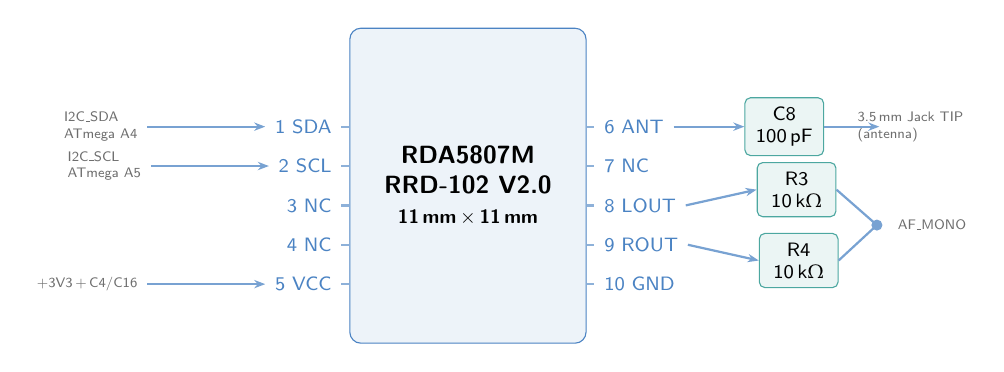
\begin{tikzpicture}[
  mod/.style={draw=accentblue!80, fill=accentblue!8, rounded corners=4pt,
              minimum width=3.0cm, minimum height=4.0cm,
              font=\sffamily\small\bfseries, align=center},
  plab/.style={font=\sffamily\scriptsize, align=right, color=accentblue!80},
  plab2/.style={font=\sffamily\scriptsize, align=left, color=accentblue!80},
  comp/.style={draw=accentteal!70, fill=accentteal!8, rounded corners=2pt,
               minimum width=1.0cm, minimum height=0.45cm,
               font=\sffamily\scriptsize, align=center},
  arr/.style={-{Stealth[length=4pt]}, thick, color=accentblue!60},
  lbl/.style={font=\sffamily\tiny, color=codegray, align=left},
  node distance=0.4cm
]
% Module body
\node[mod] (rda) {RDA5807M\\RRD-102 V2.0\\\scriptsize 11\,mm\,$\times$\,11\,mm};

% Left pins
\foreach \n/\t/\y in {1/SDA/0.75, 2/SCL/0.25, 3/NC/-0.25, 4/NC/-0.75, 5/VCC/-1.25} {
  \node[plab, left=0.1cm of rda.west, yshift=\y cm] (lp\n) {\n\ \t};
  \draw[thick, color=accentblue!50] (rda.west|-lp\n.east) -- (lp\n.east);
}
% Right pins
\foreach \n/\t/\y in {6/ANT/0.75, 7/NC/0.25, 8/LOUT/-0.25, 9/ROUT/-0.75, 10/GND/-1.25} {
  \node[plab2, right=0.1cm of rda.east, yshift=\y cm] (rp\n) {\n\ \t};
  \draw[thick, color=accentblue!50] (rda.east|-rp\n.west) -- (rp\n.west);
}

% External connections left
\node[lbl, left=1.5cm of lp1] (sda) {I2C\_SDA\\ATmega A4};
\node[lbl, left=1.5cm of lp2] (scl) {I2C\_SCL\\ATmega A5};
\node[lbl, left=1.5cm of lp5] (vcc3) {+3V3\,+\,C4/C16};
\draw[arr] (sda.east) -- (lp1.west);
\draw[arr] (scl.east) -- (lp2.west);
\draw[arr] (vcc3.east) -- (lp5.west);

% External connections right
\node[comp, right=0.9cm of rp6] (c8) {C8\\100\,pF};
\node[lbl, right=0.3cm of c8] {3.5\,mm Jack TIP\\(antenna)};
\draw[arr] (rp6.east) -- (c8.west);
\draw[arr] (c8.east) -- ++(0.7,0);

\node[comp, right=0.9cm of rp8,yshift=0.2cm] (r3) {R3\\10\,k$\Omega$};
\node[comp, right=0.9cm of rp9,yshift=-0.2cm] (r4) {R4\\10\,k$\Omega$};
\coordinate (afmix) at ($(r3.east)!0.5!(r4.east)+(0.5,0)$);
\fill[accentblue!60] (afmix) circle (2pt);
\node[lbl, right=4pt of afmix] {AF\_MONO};
\draw[arr] (rp8.east) -- (r3.west);
\draw[arr] (rp9.east) -- (r4.west);
\draw[thick, color=accentblue!60] (r3.east) -- (afmix);
\draw[thick, color=accentblue!60] (r4.east) -- (afmix);
\end{tikzpicture}
\end{diagrambox}

\subsection{PAM8403 Class-D Amplifier (SOP-16, Stereo BTL)}

The PAM8403 is a \textbf{surface-mount Class-D stereo amplifier} (SOP-16). In this design it is wired in \textbf{mono mode}: only the left input channel (INL, pin 8) receives the mono-mixed audio from R3/R4, and only the left BTL output (OUTL+/OUTL$-$) drives the 8\,$\Omega$ speaker. The right channel input (INR, pin 7) is tied to GND via a 10\,k$\Omega$ resistor to prevent noise. At VBAT 3.7\,V into 8\,$\Omega$, expect $\sim$0.5\,W output. The \textasciitilde{}SHDN pin provides \textbf{MCU-controlled mute}: ATmega D9 drives it HIGH (amplifier on) or LOW (mute when headphones detected). \textbf{SMD --- workshop solders.}

\begin{diagrambox}
\centering
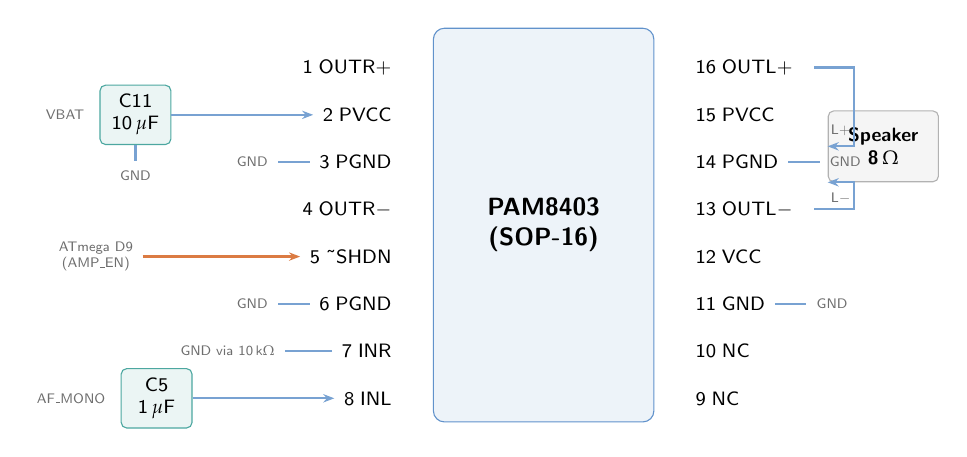
\begin{tikzpicture}[
  ic/.style={draw=accentblue!70, fill=accentblue!8,
             minimum width=2.8cm, minimum height=5.0cm,
             font=\sffamily\small\bfseries, align=center},
  pinl/.style={font=\sffamily\scriptsize, align=right},
  pinr/.style={font=\sffamily\scriptsize, align=left},
  comp/.style={draw=accentteal!70, fill=accentteal!8, rounded corners=2pt,
               minimum width=0.9cm, minimum height=0.45cm,
               font=\sffamily\scriptsize, align=center},
  arr/.style={-{Stealth[length=4pt]}, thick, color=accentblue!60},
  wire/.style={thick, color=accentblue!60},
  lbl/.style={font=\sffamily\tiny, color=codegray},
  node distance=0.15cm
]
% IC body
\node[ic, rounded corners=4pt] (pam) {PAM8403\\(SOP-16)};

% Left pin labels (1-8)
\node[pinl, left=0.4cm of pam.west, yshift= 2.0cm] (p1)  {1\;OUTR$+$};
\node[pinl, left=0.4cm of pam.west, yshift= 1.4cm] (p2)  {2\;PVCC};
\node[pinl, left=0.4cm of pam.west, yshift= 0.8cm] (p3)  {3\;PGND};
\node[pinl, left=0.4cm of pam.west, yshift= 0.2cm] (p4)  {4\;OUTR$-$};
\node[pinl, left=0.4cm of pam.west, yshift=-0.4cm] (p5)  {5\;\textasciitilde{}SHDN};
\node[pinl, left=0.4cm of pam.west, yshift=-1.0cm] (p6)  {6\;PGND};
\node[pinl, left=0.4cm of pam.west, yshift=-1.6cm] (p7)  {7\;INR};
\node[pinl, left=0.4cm of pam.west, yshift=-2.2cm] (p8)  {8\;INL};

% Right pin labels (16-9)
\node[pinr, right=0.4cm of pam.east, yshift= 2.0cm] (p16) {16\;OUTL$+$};
\node[pinr, right=0.4cm of pam.east, yshift= 1.4cm] (p15) {15\;PVCC};
\node[pinr, right=0.4cm of pam.east, yshift= 0.8cm] (p14) {14\;PGND};
\node[pinr, right=0.4cm of pam.east, yshift= 0.2cm] (p13) {13\;OUTL$-$};
\node[pinr, right=0.4cm of pam.east, yshift=-0.4cm] (p12) {12\;VCC};
\node[pinr, right=0.4cm of pam.east, yshift=-1.0cm] (p11) {11\;GND};
\node[pinr, right=0.4cm of pam.east, yshift=-1.6cm] (p10) {10\;NC};
\node[pinr, right=0.4cm of pam.east, yshift=-2.2cm] (p9)  {9\;NC};

% Speaker on right (bridged)
\node[draw=gray!60, fill=gray!8, rounded corners=2pt,
      right=2.2cm of pam.east, yshift=1.0cm, minimum width=1.4cm, minimum height=0.9cm,
      font=\sffamily\scriptsize\bfseries, align=center] (spk) {Speaker\\8\,$\Omega$};
\draw[arr] (p16.east) ++(0.15,0) -- ++(0.5,0) |- node[lbl,near end,above]{L$+$} (spk.west);
\draw[arr] (p13.east) ++(0.15,0) -- ++(0.5,0) |- node[lbl,near end,below]{L$-$} (spk.south west);

% PVCC and bypass
\node[comp, left=1.8cm of p2] (c11) {C11\\10\,$\mu$F};
\draw[arr] (c11.east) -- (p2.west);
\node[lbl, left=2pt of c11] {VBAT};
\draw[wire] (c11.south) -- ++(0,-0.2) node[lbl,below]{GND};

% SHDN from MCU
\node[lbl, left=2.0cm of p5, align=center] (shdn) {ATmega D9\\(AMP\_EN)};
\draw[arr, color=accentorange!80] (shdn.east) -- (p5.west);

% Audio input (mono to INL only, INR to GND)
\node[comp, left=1.8cm of p8] (c5l) {C5\\1\,$\mu$F};
\node[lbl, left=2pt of c5l] {AF\_MONO};
\draw[arr] (c5l.east) -- (p8.west);
\draw[wire] (p7.west) -- ++(-0.6,0) node[lbl,left]{GND via 10\,k$\Omega$};

% GND pins
\draw[wire] (p3.west) -- ++(-0.4,0) node[lbl,left]{GND};
\draw[wire] (p6.west) -- ++(-0.4,0) node[lbl,left]{GND};
\draw[wire] (p11.east) -- ++(0.4,0) node[lbl,right]{GND};
\draw[wire] (p14.east) -- ++(0.4,0) node[lbl,right]{GND};

\end{tikzpicture}
\end{diagrambox}

\begin{infobox}
\textbf{PAM8403 connections (stereo BTL):}
\begin{itemize}[noitemsep]
  \item \textbf{PVCC (pins 2, 15)} $\leftarrow$ VBAT direct + C11 (10\,$\mu$F ceramic) on pin 2 + C20 (10\,$\mu$F ceramic) on pin 15. Each PVCC pin requires its own local bypass cap.
  \item \textbf{VCC (pin 12)} $\leftarrow$ VBAT (logic supply)
  \item \textbf{PGND (pins 3, 6, 14)} and \textbf{GND (pin 11)} $\rightarrow$ GND plane (wide traces, short path)
  \item \textbf{INL (pin 8)} $\leftarrow$ C5 (1\,$\mu$F) from mono-mixed AF\_MONO (R3+R4 sum of LOUT+ROUT)
  \item \textbf{INR (pin 7)} $\rightarrow$ tied to GND via 10\,k$\Omega$ (unused; prevents noise pickup)
  \item \textbf{OUTL+/OUTL$-$ (pins 16, 13)} $\rightarrow$ Speaker (BTL --- neither wire to GND)
  \item \textbf{OUTR+/OUTR$-$ (pins 1, 4)} $\rightarrow$ unused (no connection, or leave NC)
  \item \textbf{\textasciitilde{}SHDN (pin 5)} $\leftarrow$ ATmega D9. HIGH = amplifier on. LOW = shutdown (mute).
\end{itemize}
\textbf{MCU-controlled speaker mute}: When headphones are detected on D8, the MCU pulls D9 LOW to assert \textasciitilde{}SHDN, shutting down the PAM8403. When headphones are removed, D9 goes HIGH and the speaker resumes.
\end{infobox}

\begin{warningbox}
PAM8403 outputs are BTL (Bridge-Tied Load). \textbf{Neither speaker wire goes to GND.} Connecting either speaker wire to ground will damage the IC. The speaker floats between OUTL+ and OUTL$-$.
\end{warningbox}

\subsection{3.5\,mm Headphone Jack}

\begin{diagrambox}
\centering
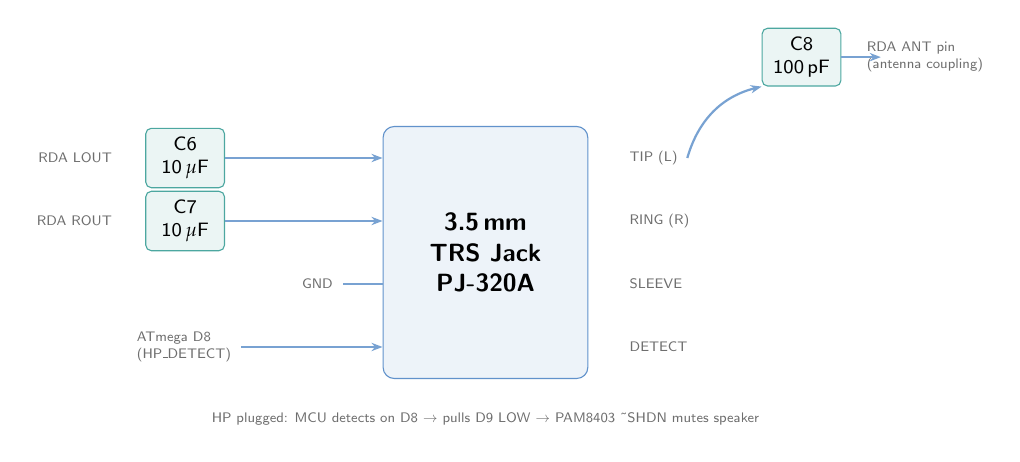
\begin{tikzpicture}[
  jack/.style={draw=accentblue!70, fill=accentblue!8, rounded corners=4pt,
               minimum width=2.6cm, minimum height=3.2cm, align=center,
               font=\sffamily\small\bfseries},
  comp/.style={draw=accentteal!70, fill=accentteal!8, rounded corners=2pt,
               minimum width=1.0cm, minimum height=0.45cm,
               font=\sffamily\scriptsize, align=center},
  arr/.style={-{Stealth[length=4pt]}, thick, color=accentblue!60},
  wire/.style={thick, color=accentblue!60},
  lbl/.style={font=\sffamily\tiny, color=codegray, align=left},
  node distance=0.4cm
]
\node[jack] (j) {3.5\,mm\\TRS Jack\\PJ-320A};

% Pins on the right
\node[lbl, right=0.4cm of j.east, yshift= 1.2cm] (tip)    {TIP (L)};
\node[lbl, right=0.4cm of j.east, yshift= 0.4cm] (ring)   {RING (R)};
\node[lbl, right=0.4cm of j.east, yshift=-0.4cm] (sleeve) {SLEEVE};
\node[lbl, right=0.4cm of j.east, yshift=-1.2cm] (det)    {DETECT};

% Connections left (sources)
\node[comp, left=2.0cm of j.west, yshift= 1.2cm] (c6)  {C6\\10\,$\mu$F};
\node[comp, left=2.0cm of j.west, yshift= 0.4cm] (c7)  {C7\\10\,$\mu$F};
\node[lbl,  left=1.8cm of j.west, yshift=-1.2cm] (d8) {ATmega D8\\(HP\_DETECT)};

\node[lbl, left=0.3cm of c6] {RDA LOUT};
\node[lbl, left=0.3cm of c7] {RDA ROUT};

\draw[arr] (c6.east)  -- (j.west|-c6);
\draw[arr] (c7.east)  -- (j.west|-c7);
\draw[wire] (j.west|-sleeve.center) -- ++(-0.5,0) node[lbl,left]{GND};
\draw[arr] (d8.east)  -- (j.west|-d8);

% Antenna coupling
\node[comp, above right=0.5cm and 2.2cm of j.north east] (c8) {C8\\100\,pF};
\node[lbl, right=0.2cm of c8] {RDA ANT pin\\(antenna coupling)};
\draw[arr, bend left=30] (tip.east) to (c8.south west);
\draw[arr] (c8.east) -- ++(0.5,0);

% Note
\node[lbl, below=0.3cm of j.south] {HP plugged: MCU detects on D8 $\to$ pulls D9 LOW $\to$ PAM8403 \textasciitilde{}SHDN mutes speaker};

\end{tikzpicture}
\end{diagrambox}

\subsection{I2C Bus}

\begin{diagrambox}
\centering
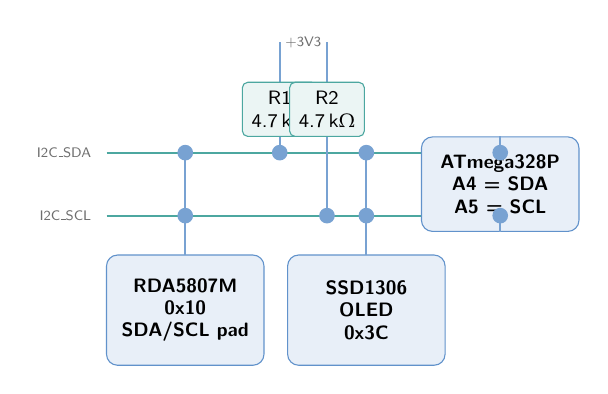
\begin{tikzpicture}[
  ic/.style={draw=accentblue!70, fill=accentblue!10, rounded corners=4pt,
             minimum width=2.0cm, minimum height=1.0cm,
             font=\sffamily\scriptsize\bfseries, align=center},
  comp/.style={draw=accentteal!70, fill=accentteal!8, rounded corners=2pt,
               minimum width=0.8cm, minimum height=0.45cm,
               font=\sffamily\scriptsize, align=center},
  arr/.style={-{Stealth[length=4pt]}, thick, color=accentblue!60},
  wire/.style={thick, color=accentblue!60},
  bus/.style={thick, color=accentteal!70},
  lbl/.style={font=\sffamily\tiny, color=codegray},
  dot/.style={fill=accentblue!60, circle, inner sep=2pt}
]
% Pull-up resistors
\node[lbl] (vcc) at (2.5,3.2) {+3V3};
\draw[wire] (2.2,3.2) -- (2.2,2.7);
\draw[wire] (2.8,3.2) -- (2.8,2.7);
\node[comp] (r1) at (2.2, 2.35) {R1\\4.7\,k$\Omega$};
\node[comp] (r2) at (2.8, 2.35) {R2\\4.7\,k$\Omega$};

% SDA line
\draw[bus] (0,1.8) -- (5.5,1.8);
\node[lbl, left=2pt] at (0,1.8) {I2C\_SDA};
\draw[wire] (r1.south) -- (2.2,1.8);
\node[dot] at (2.2,1.8) {};

% SCL line
\draw[bus] (0,1.0) -- (5.5,1.0);
\node[lbl, left=2pt] at (0,1.0) {I2C\_SCL};
\draw[wire] (r2.south) -- (2.8,1.0);
\node[dot] at (2.8,1.0) {};

% ATmega
\node[ic, minimum height=1.2cm, minimum width=2.0cm] (mcu) at (5.0,1.4) {ATmega328P\\A4 = SDA\\A5 = SCL};
\draw[wire] (5.0,1.8) -- (mcu.north-|5.0,1.8);
\draw[wire] (5.0,1.0) -- (mcu.south-|5.0,1.0);
\node[dot] at (5.0,1.8) {};
\node[dot] at (5.0,1.0) {};

% RDA5807M
\node[ic, minimum height=1.4cm] (rda) at (1.0,-0.2) {RDA5807M\\0x10\\SDA/SCL pad};
\draw[wire] (1.0,1.8) -- (rda.north-|1.0,0);
\draw[wire] (1.0,1.0) -- (1.0,0.5);
\node[dot] at (1.0,1.8) {};
\node[dot] at (1.0,1.0) {};

% SSD1306
\node[ic, minimum height=1.4cm] (oled) at (3.3,-0.2) {SSD1306\\OLED\\0x3C};
\draw[wire] (3.3,1.8) -- (oled.north-|3.3,0);
\draw[wire] (3.3,1.0) -- (3.3,0.5);
\node[dot] at (3.3,1.8) {};
\node[dot] at (3.3,1.0) {};

\end{tikzpicture}
\end{diagrambox}

\subsection{Rotary Encoders}

\begin{diagrambox}
\centering
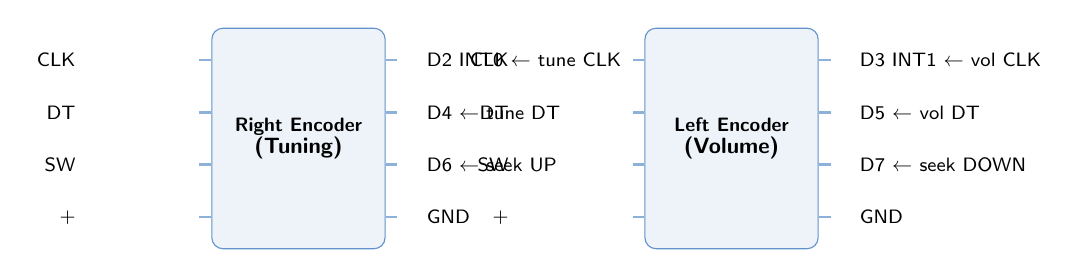
\begin{tikzpicture}[
  enc/.style={draw=accentblue!70, fill=accentblue!8, rounded corners=4pt,
              minimum width=2.2cm, minimum height=2.8cm,
              font=\sffamily\scriptsize\bfseries, align=center},
  pin/.style={font=\sffamily\scriptsize, align=right},
  pin2/.style={font=\sffamily\scriptsize, align=left},
  arr/.style={-{Stealth[length=4pt]}, thick, color=accentblue!60},
  lbl/.style={font=\sffamily\tiny, color=codegray},
  node distance=0.3cm
]
% Right encoder
\node[enc] (renc) at (0,0) {Right Encoder\\\footnotesize(Tuning)};
\node[pin, left=1.6cm of renc.west, yshift= 1.0cm] (rclk) {CLK};
\node[pin, left=1.6cm of renc.west, yshift= 0.33cm] (rdt)  {DT};
\node[pin, left=1.6cm of renc.west, yshift=-0.33cm] (rsw)  {SW};
\node[pin, left=1.6cm of renc.west, yshift=-1.0cm] (rvcc) {+};

\node[pin2, right=0.4cm of renc.east, yshift= 1.0cm] {D2 INT0 $\leftarrow$ tune CLK};
\node[pin2, right=0.4cm of renc.east, yshift= 0.33cm] {D4 $\leftarrow$ tune DT};
\node[pin2, right=0.4cm of renc.east, yshift=-0.33cm] {D6 $\leftarrow$ seek UP};
\node[pin2, right=0.4cm of renc.east, yshift=-1.0cm] {GND};

\foreach \p/\y in {rclk/1.0, rdt/0.33, rsw/-0.33, rvcc/-1.0} {
  \draw[thick, accentblue!50] (renc.west|-\p.east) -- ++(-0.15,0);
  \draw[thick, accentblue!50] (renc.east) ++(0,\y cm) -- ++(0.15,0);
}

% Left encoder
\node[enc] (lenc) at (5.5,0) {Left Encoder\\\footnotesize(Volume)};
\node[pin, left=1.6cm of lenc.west, yshift= 1.0cm] (lclk) {CLK};
\node[pin, left=1.6cm of lenc.west, yshift= 0.33cm] (ldt)  {DT};
\node[pin, left=1.6cm of lenc.west, yshift=-0.33cm] (lsw)  {SW};
\node[pin, left=1.6cm of lenc.west, yshift=-1.0cm] (lvcc) {+};

\node[pin2, right=0.4cm of lenc.east, yshift= 1.0cm] {D3 INT1 $\leftarrow$ vol CLK};
\node[pin2, right=0.4cm of lenc.east, yshift= 0.33cm] {D5 $\leftarrow$ vol DT};
\node[pin2, right=0.4cm of lenc.east, yshift=-0.33cm] {D7 $\leftarrow$ seek DOWN};
\node[pin2, right=0.4cm of lenc.east, yshift=-1.0cm] {GND};

\foreach \p/\y in {lclk/1.0, ldt/0.33, lsw/-0.33, lvcc/-1.0} {
  \draw[thick, accentblue!50] (lenc.west|-\p.east) -- ++(-0.15,0);
  \draw[thick, accentblue!50] (lenc.east) ++(0,\y cm) -- ++(0.15,0);
}
\end{tikzpicture}
\end{diagrambox}

\subsection{Programming Interface (CH340C + USB-C)}

The CH340C is a \textbf{surface-mount USB-to-serial bridge} (SOP-16) permanently soldered on the PCB by the university workshop. It connects the USB-C data lines (D+/D$-$) to the ATmega UART (D0/D1), allowing firmware upload directly via the same USB-C port used for charging. No external crystal is needed --- the CH340C has an internal oscillator.

\begin{warningbox}
\textbf{CH340C V3 pin (pin 4):} This pin \textbf{must} be connected to +3V3 via a 100\,nF bypass capacitor (C18) to GND. The V3 pin is the internal regulator output and \textbf{must not be left floating}---the chip will not enumerate on USB without it. At 3.3\,V VCC, tie V3 directly to VCC and add C18 (100\,nF) from V3 to GND.
\end{warningbox}

\begin{diagrambox}
\centering
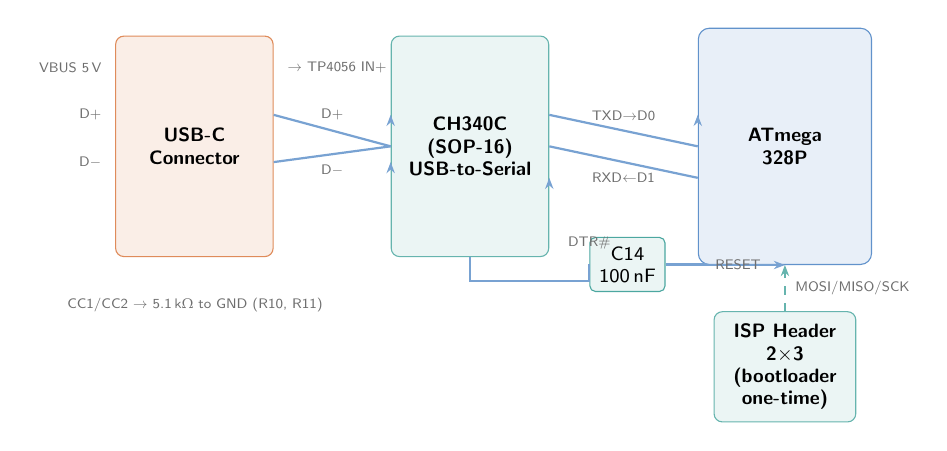
\begin{tikzpicture}[
  mcu/.style={draw=accentblue!70, fill=accentblue!10, rounded corners=4pt,
              minimum width=2.2cm, minimum height=3.0cm,
              font=\sffamily\scriptsize\bfseries, align=center},
  hdr/.style={draw=accentteal!60, fill=accentteal!8, rounded corners=3pt,
              minimum width=2.0cm, minimum height=2.8cm,
              font=\sffamily\scriptsize\bfseries, align=center},
  isp/.style={draw=accentteal!60, fill=accentteal!8, rounded corners=3pt,
              minimum width=1.8cm, minimum height=1.4cm,
              font=\sffamily\scriptsize\bfseries, align=center},
  comp/.style={draw=accentteal!70, fill=accentteal!8, rounded corners=2pt,
               minimum width=0.8cm, minimum height=0.4cm,
               font=\sffamily\scriptsize, align=center},
  arr/.style={-{Stealth[length=4pt]}, thick, color=accentblue!60},
  wire/.style={thick, color=accentblue!60},
  lbl/.style={font=\sffamily\tiny, color=codegray},
  node distance=0.6cm and 1.4cm
]
% USB-C port
\node[hdr, fill=accentorange!10, draw=accentorange!70] (usbc) at (0,0) {USB-C\\Connector};
\node[lbl, left=0.05cm of usbc.west, yshift= 1.0cm] {VBUS 5\,V};
\node[lbl, left=0.05cm of usbc.west, yshift= 0.4cm] {D+};
\node[lbl, left=0.05cm of usbc.west, yshift=-0.2cm] {D$-$};
\node[lbl, right=0.05cm of usbc.east, yshift= 1.0cm] {$\to$ TP4056 IN+};

% CH340C
\node[hdr] (ch340) at (3.5,0) {CH340C\\(SOP-16)\\USB-to-Serial};

% ATmega
\node[mcu] (mcu) at (7.5,0) {ATmega\\328P};

% ISP header
\node[isp] (isp) at (7.5,-2.8) {ISP Header\\2$\times$3\\(bootloader\\one-time)};

% Auto-reset cap
\node[comp] (c14) at (5.5,-1.5) {C14\\100\,nF};

% USB-C to CH340C
\draw[arr] (usbc.east) ++(0, 0.4) -- node[lbl,above]{D+} (ch340.west|-usbc.east) ++(0,0.4);
\draw[arr] (usbc.east) ++(0,-0.2) -- node[lbl,below]{D$-$} (ch340.west|-usbc.east) ++(0,-0.2);

% CH340C to ATmega UART
\draw[arr] (ch340.east) ++(0, 0.4) -- node[lbl,above]{TXD$\to$D0} (mcu.west) ++(0,0.4);
\draw[arr] (mcu.west) ++(0,-0.4) -- node[lbl,below]{RXD$\leftarrow$D1} (ch340.east) ++(0,-0.4);

% Auto-reset
\draw[wire] (ch340.south) -- ++(0,-0.3) -| (c14.west);
\node[lbl, above=2pt of c14.west] {DTR\#};
\draw[arr] (c14.east) -- ++(0.5,0) |- node[lbl,right]{RESET} (mcu.south);

% ISP to ATmega
\draw[arr,dashed,accentteal!60] (isp.north) -- node[lbl,right]{MOSI/MISO/SCK} (mcu.south);

% CC pulldowns
\node[lbl, below=0.4cm of usbc, text width=4cm, align=center] {CC1/CC2 $\to$ 5.1\,k$\Omega$ to GND (R10, R11)};

\end{tikzpicture}
\end{diagrambox}

\begin{infobox}
\textbf{Two-step programming workflow:}
\begin{enumerate}[noitemsep]
  \item \textbf{One time only (bootloader):} Use an Arduino UNO as ISP (ArduinoISP sketch) connected to the 2$\times$3 ISP header (J3). This burns the Arduino Pro Mini 3.3\,V 8\,MHz bootloader.
  \item \textbf{Every firmware upload:} Plug a USB-C cable from your PC into J4. In Arduino IDE select ``Arduino Pro Mini'' $\to$ ``3.3\,V, 8\,MHz'' and the CH340 COM port. Upload as normal. Auto-reset via CH340C DTR\# + C14 works the same as on any Arduino Pro Mini.
\end{enumerate}
\textbf{CH340C driver:} Windows 10/11 usually auto-installs. If not, download the CH340 driver from WCH's website (free, one-time install).
\end{infobox}

\subsection{Battery Voltage Divider}

\begin{diagrambox}
\centering
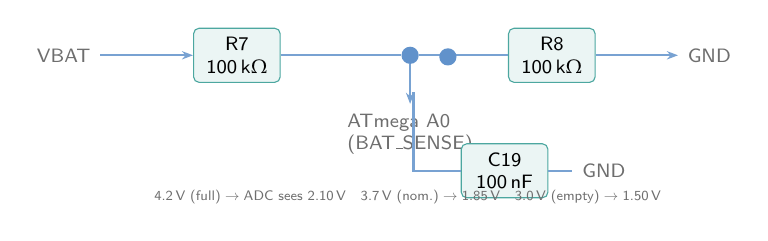
\begin{tikzpicture}[
  comp/.style={draw=accentteal!70, fill=accentteal!8, rounded corners=2pt,
               minimum width=1.1cm, minimum height=0.5cm,
               font=\sffamily\scriptsize, align=center},
  arr/.style={-{Stealth[length=4pt]}, thick, color=accentblue!60},
  wire/.style={thick, color=accentblue!60},
  lbl/.style={font=\sffamily\scriptsize, color=codegray, align=left},
  dot/.style={fill=accentblue!70, circle, inner sep=2.2pt}
]
% VBAT source
\node[lbl] (vbat) at (0,0) {VBAT};
\node[comp] (r7) at (2.2,0) {R7\\100\,k$\Omega$};
\node[dot] (mid) at (4.4,0) {};
\node[comp] (r8) at (6.2,0) {R8\\100\,k$\Omega$};
\node[lbl] (gnd) at (8.2,0) {GND};
\node[lbl, below=0.5cm of mid] (a0) {ATmega A0\\(BAT\_SENSE)};
\node[comp, below=1.0cm of mid, xshift=1.2cm] (c19) {C19\\100\,nF};
% Wires
\draw[arr] (vbat.east) -- (r7.west);
\draw[wire] (r7.east) -- (mid);
\draw[wire] (mid) -- (r8.west);
\draw[arr] (r8.east) -- (gnd.west);
\draw[arr] (mid) -- (a0.north);
\draw[wire] (c19.west) -- ++(-0.6,0) -- ++(0,1.0);
\node[dot] at (4.88,-0.02) {};
\draw[wire] (c19.east) -- ++(0.3,0) node[lbl,right]{GND};
% Table
\node[align=left, font=\sffamily\tiny, color=codegray] at (4.4,-1.8) {
  4.2\,V (full)\;$\rightarrow$\;ADC sees 2.10\,V\quad
  3.7\,V (nom.)\;$\rightarrow$\;1.85\,V\quad
  3.0\,V (empty)\;$\rightarrow$\;1.50\,V
};
\end{tikzpicture}
\end{diagrambox}

\subsection{Power LED}

\begin{diagrambox}
\centering
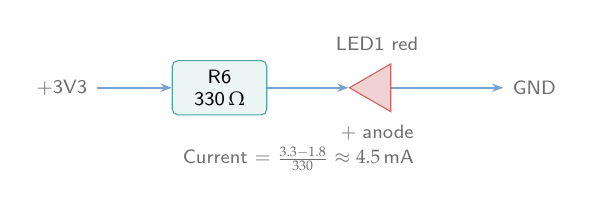
\begin{tikzpicture}[
  comp/.style={draw=accentteal!70, fill=accentteal!8, rounded corners=2pt,
               minimum width=1.2cm, minimum height=0.5cm,
               font=\sffamily\scriptsize, align=center},
  led/.style={draw=accentred!70, fill=accentred!20, regular polygon,
              regular polygon sides=3, shape border rotate=90,
              minimum size=0.7cm, font=\sffamily\tiny, inner sep=0pt},
  wire/.style={thick, color=accentblue!60},
  arr/.style={-{Stealth[length=4pt]}, thick, color=accentblue!60},
  lbl/.style={font=\sffamily\scriptsize, color=codegray}
]
\node[lbl] (vcc) at (0,0) {+3V3};
\node[comp] (r6) at (2.0,0) {R6\\330\,$\Omega$};
\node[led] (led1) at (4.0,0) {};
\node[lbl, above=4pt of led1] {LED1 red};
\node[lbl, below=4pt of led1] {$+$\;anode};
\node[lbl] (gnd) at (6.0,0) {GND};
\draw[arr] (vcc.east) -- (r6.west);
\draw[arr] (r6.east) -- (led1.west);
\draw[arr] (led1.east) -- (gnd.west);
\node[lbl] at (3.0,-0.9) {Current $= \frac{3.3 - 1.8}{330} \approx 4.5$\,mA};
\end{tikzpicture}
\end{diagrambox}

\subsection{Complete Connection Checklist}

Use this as a verification checklist. Every wire in the project:

\begin{longtable}{@{}p{0.5cm}p{5cm}p{5cm}p{1.5cm}@{}}
\toprule
\textbf{\#} & \textbf{From} & \textbf{To} & \textbf{Check} \\
\midrule
\endhead
1 & ATmega pin 1 (RESET) & R5 (10\,k$\Omega$) to +3V3, ISP pin 5, C14 (100\,nF) to CH340C DTR\# & $\square$ \\
2 & ATmega pin 2 (D0/RX) & CH340C TXD & $\square$ \\
3 & ATmega pin 3 (D1/TX) & CH340C RXD & $\square$ \\
4 & ATmega pin 4 (D2) & Right encoder CLK & $\square$ \\
5 & ATmega pin 5 (D3) & Left encoder CLK & $\square$ \\
6 & ATmega pin 6 (D4) & Right encoder DT & $\square$ \\
7 & ATmega pin 7 (VCC) & +3V3 + C1(100nF) to GND & $\square$ \\
8 & ATmega pin 8 (GND) & GND bus & $\square$ \\
9 & ATmega pin 9 (XTAL1) & Y1 leg 1 + C3a(22pF) to GND & $\square$ \\
10 & ATmega pin 10 (XTAL2) & Y1 leg 2 + C3b(22pF) to GND & $\square$ \\
11 & ATmega pin 11 (D5) & Left encoder DT & $\square$ \\
12 & ATmega pin 12 (D6) & Right encoder SW & $\square$ \\
13 & ATmega pin 13 (D7) & Left encoder SW & $\square$ \\
14 & ATmega pin 14 (D8) & 3.5mm jack DETECT pin (HP\_DET) & $\square$ \\
15 & ATmega pin 15 (D9) & PAM8403 \textasciitilde{}SHDN (AMP\_EN: HIGH=on, LOW=mute) & $\square$ \\
16 & ATmega pin 17 (D11) & ISP header pin 4 (MOSI) & $\square$ \\
17 & ATmega pin 18 (D12) & ISP header pin 1 (MISO) & $\square$ \\
18 & ATmega pin 19 (D13) & ISP header pin 3 (SCK) & $\square$ \\
19 & ATmega pin 20 (AVCC) & +3V3 + C2(100nF) to GND & $\square$ \\
20 & ATmega pin 22 (AGND) & GND bus & $\square$ \\
20b & ATmega pin 21 (AREF) & C21 (100\,nF) to GND (ADC reference filter) & $\square$ \\
21 & ATmega pin 23 (A0) & R7/R8 divider midpoint + C19 (100\,nF) to GND & $\square$ \\
22 & ATmega pin 27 (A4/SDA) & I2C\_SDA bus & $\square$ \\
23 & ATmega pin 28 (A5/SCL) & I2C\_SCL bus & $\square$ \\
24 & R1(4.7k) & I2C\_SDA to +3V3 & $\square$ \\
25 & R2(4.7k) & I2C\_SCL to +3V3 & $\square$ \\
26 & RDA5807M pad 1 (SDA) & I2C\_SDA bus & $\square$ \\
27 & RDA5807M pad 2 (SCL) & I2C\_SCL bus & $\square$ \\
28 & RDA5807M pad 5 (VCC) & +3V3 + C4(100nF) + C16(10uF) & $\square$ \\
29 & RDA5807M pad 6 (ANT) & C8(100pF) to jack TIP + J9 pad & $\square$ \\
30 & RDA5807M pad 8 (LOUT) & R3(10k) to AF\_MONO mix point; also C6(10$\mu$F) to jack TIP (stereo HP) & $\square$ \\
31 & RDA5807M pad 9 (ROUT) & R4(10k) to AF\_MONO mix point; also C7(10$\mu$F) to jack RING (stereo HP) & $\square$ \\
32 & RDA5807M pad 10 (GND) & GND bus & $\square$ \\
33 & SSD1306 GND & GND bus & $\square$ \\
34 & SSD1306 VCC & +3V3 & $\square$ \\
35 & SSD1306 SCL & I2C\_SCL bus & $\square$ \\
36 & SSD1306 SDA & I2C\_SDA bus & $\square$ \\
37 & PAM8403 INL (pin 8) & C5 (1\,$\mu$F) from AF\_MONO mix point (R3+R4 junction) & $\square$ \\
38 & PAM8403 INR (pin 7) & Tied to GND via 10\,k$\Omega$ (unused; mono speaker only) & $\square$ \\
39 & PAM8403 PVCC (pins 2, 15) & VBAT + C11 (10\,$\mu$F) on pin 2 + C20 (10\,$\mu$F) on pin 15 --- each PVCC needs its own bypass & $\square$ \\
40 & PAM8403 VCC (pin 12) & VBAT (logic supply) & $\square$ \\
41 & PAM8403 PGND (pins 3, 6, 14) & GND plane (wide trace, multiple vias) & $\square$ \\
42 & PAM8403 GND (pin 11) & GND plane & $\square$ \\
43 & PAM8403 OUTL+ (pin 16) & Speaker$+$ (SPK+ terminal J8) & $\square$ \\
44 & PAM8403 OUTL$-$ (pin 13) & Speaker$-$ (SPK$-$ terminal J8) & $\square$ \\
45 & PAM8403 \textasciitilde{}SHDN (pin 5) & ATmega D9 (AMP\_EN) & $\square$ \\
46 & 3.5\,mm jack TIP & C6 from LOUT + C8 to RDA ANT & $\square$ \\
47 & 3.5\,mm jack RING & C7 from ROUT & $\square$ \\
48 & 3.5\,mm jack SLEEVE & GND & $\square$ \\
49 & 3.5\,mm jack DETECT & ATmega D8 (HP\_DET) & $\square$ \\
50 & USB-C VBUS & TP4056 VCC (pin 4) + C12 bypass & $\square$ \\
51 & USB-C D+ & CH340C UD+ & $\square$ \\
52 & USB-C D$-$ & CH340C UD$-$ & $\square$ \\
53 & USB-C CC1 & R10 (5.1\,k$\Omega$) to GND & $\square$ \\
54 & USB-C CC2 & R11 (5.1\,k$\Omega$) to GND & $\square$ \\
55 & USB-C GND & GND bus & $\square$ \\
56 & CH340C TXD & ATmega pin 2 (D0/RX) & $\square$ \\
57 & CH340C RXD & ATmega pin 3 (D1/TX) & $\square$ \\
58 & CH340C DTR\# & C14 (100\,nF) to ATmega RESET (auto-reset) & $\square$ \\
59 & CH340C VCC & +3V3 + C13 (100\,nF) bypass & $\square$ \\
59b & CH340C V3 (pin 4) & +3V3 + C18 (100\,nF) bypass to GND --- required for USB enumeration & $\square$ \\
60 & TP4056 BAT (pin 3) & DW01A $\to$ LiPo J2 positive + C17 (1$\mu$F) & $\square$ \\
61 & TP4056 PROG (pin 2) & R9 (2.2\,k$\Omega$) to GND ($\sim$455\,mA charge current) & $\square$ \\
62 & TP4056 CHRG (pin 7) & VBUS $\to$ R12 (1\,k$\Omega$) $\to$ LED2 (red anode) $\to$ CHRG pin 7 (open-drain sink) & $\square$ \\
63 & TP4056 STDBY (pin 6) & VBUS $\to$ R13 (1\,k$\Omega$) $\to$ LED3 (green anode) $\to$ STDBY pin 6 (open-drain sink) & $\square$ \\
64 & DW01A/FS8205A & Low-side on BAT$-$ path: LiPo BAT$-$ $\to$ FS8205A drain; FS8205A source $\to$ R14 (100$\Omega$) $\to$ GND. DW01A CS pin to midpoint. Protects against over-discharge/over-charge/short-circuit. & $\square$ \\
65 & TP4056 BAT+ (via latching SW1) & SW1 input $\to$ VBAT bus. DW01A/FS8205A is on BAT$-$ (low-side), NOT on BAT+. & $\square$ \\
66 & SW1 output & VBAT bus & $\square$ \\
67 & VBAT & HT7333 IN + PAM8403 PVCC + R7 (100\,k$\Omega$) & $\square$ \\
68 & HT7333 OUT & +3V3 bus + C9 (in) + C10 (out) bypasses & $\square$ \\
69 & Power LED & +3V3 $-$ R6 (330\,$\Omega$) $-$ LED1 $-$ GND & $\square$ \\
\bottomrule
\end{longtable}

% ============================================================================
\section{KiCad 9.0 --- Schematic Entry (Step by Step)}
\label{sec:kicad-sch}
% ============================================================================

\subsection{Opening the Project}

\begin{enumerate}
    \item Open KiCad 9.0
    \item File $\rightarrow$ Open Project $\rightarrow$ navigate to \texttt{ESP32\_FM\_Radio\_V2/}
    \item Double-click the \texttt{.kicad\_sch} file to open the schematic editor
    \item The schematic is blank --- we start from scratch
\end{enumerate}

\begin{infobox}
Optional: Rename the project folder to something like \texttt{FM\_Pocket\_Radio\_V3/} to avoid confusion with the old ESP32 project name.
\end{infobox}

\subsection{Setting Up Schematic Sheets}

For a clean layout, use one sheet with logical grouping:
\begin{itemize}[noitemsep]
    \item Top-left: Power supply (USB-C + TP4056 + DW01A + HT7333 + switch)
    \item Top-right: MCU (ATmega328P + crystal + CH340C + ISP header)
    \item Bottom-left: Radio (RDA5807M + I2C + antenna)
    \item Bottom-right: Audio (PAM8403 + speaker + headphone jack)
    \item Center: Display + encoders
\end{itemize}

\subsection{Placing Components}

Press \textbf{A} (Add Symbol) to place components. Search by name:

\begin{longtable}{@{}p{5cm}p{4cm}p{4cm}@{}}
\toprule
\textbf{Component} & \textbf{KiCad Library} & \textbf{Symbol Name} \\
\midrule
\endhead
ATmega328P-PU & MCU\_Microchip\_ATmega & ATmega328P-PU \\
ATmega328P-AU (alt.) & MCU\_Microchip\_ATmega & ATmega328P-AU \\
Crystal 8\,MHz & Device & Crystal \\
Resistor & Device & R \\
Capacitor & Device & C \\
Capacitor polarized & Device & C\_Polarized \\
LED & Device & LED \\
Power flag & power & PWR\_FLAG \\
+3V3 & power & +3V3 \\
GND & power & GND \\
\midrule
\multicolumn{3}{l}{\textit{Custom symbols (must import --- see Section~\ref{sec:import}):}} \\
RDA5807M module & Custom lib & RDA5807M\_Module \\
PAM8403 & Custom lib & PAM8403 \\
TP4056 IC (SOP-8) & Custom lib & TP4056 \\
CH340C & Custom lib & CH340C \\
HT7333 (SOT-89) & Custom lib & HT7333 \\
DW01A + FS8205A & Custom lib & DW01A / FS8205A \\
USB-C connector & Connector\_USB & USB\_C\_Receptacle\_USB2.0 \\
SSD1306 OLED & Custom lib & SSD1306\_Module \\
3.5\,mm Audio Jack & Connector\_Audio & AudioJack3\_SwitchT \\
Rotary Encoder & Device & RotaryEncoder\_Switch \\
\bottomrule
\end{longtable}

\subsection{Wiring}

\begin{enumerate}
    \item Press \textbf{W} to start a wire
    \item Connect pins as per the connection table in Section~\ref{sec:circuit}
    \item Use \textbf{labels} (press \textbf{L}) for long-distance connections: \texttt{I2C\_SDA}, \texttt{I2C\_SCL}, \texttt{+3V3}, \texttt{VBAT}, \texttt{AF\_MONO}, etc.
    \item Add \textbf{power flags}: place \texttt{PWR\_FLAG} symbols on +3V3 and GND to avoid ERC warnings
    \item Add net labels on all signal wires for clarity
\end{enumerate}

\subsection{Annotation and Values}

\begin{enumerate}
    \item Edit $\rightarrow$ Annotate Schematic (or press \textbf{Ctrl+Shift+A})
    \item Assigns R1, R2, C1, C2, U1, etc. automatically
    \item Double-click each component to set its \textbf{Value}: ``4.7k'', ``100nF'', ``ATmega328P-PU'', etc.
\end{enumerate}

\subsection{Running ERC}

\begin{enumerate}
    \item Inspect $\rightarrow$ Electrical Rules Checker (or toolbar icon)
    \item Click ``Run ERC''
    \item Fix all errors. Common issues:
    \begin{itemize}[noitemsep]
        \item Missing power flags on power rails --- add PWR\_FLAG symbols
        \item Unconnected pins --- add ``no connect'' flags (press \textbf{Q})
        \item Pin type conflicts --- verify power pin directions
    \end{itemize}
    \item \textbf{Zero errors required} before proceeding to PCB layout
\end{enumerate}

% ============================================================================
\section{Importing Custom Components in KiCad 9.0}
\label{sec:import}
% ============================================================================

Several components are NOT in KiCad's default libraries. You must import or create them.

\subsection{Method 1: Download from SnapEDA (Recommended)}

\begin{enumerate}
    \item Go to \url{https://www.snapeda.com}
    \item Search for the component (e.g., ``PAM8403'', ``CH340C'', ``RDA5807M'')
    \item Click ``Download Symbol \& Footprint''
    \item Select ``KiCad'' format
    \item Download the ZIP file
    \item Extract --- you get \texttt{.kicad\_sym} (symbol) and \texttt{.kicad\_mod} (footprint) files
    \item \textbf{Place files:} Create a folder \texttt{libs/} inside your KiCad project directory. Copy the downloaded files there.
\end{enumerate}

\subsubsection{Register Symbol Library}
\begin{enumerate}
    \item In KiCad Schematic Editor: Preferences $\rightarrow$ Manage Symbol Libraries
    \item Click the \textbf{Project Specific Libraries} tab
    \item Click the ``+'' (add) button
    \item For ``Library Path'', browse to your \texttt{libs/something.kicad\_sym} file
    \item Give it a nickname (e.g., ``PAM8403'')
    \item Click OK
\end{enumerate}

\subsubsection{Register Footprint Library}
\begin{enumerate}
    \item In KiCad PCB Editor: Preferences $\rightarrow$ Manage Footprint Libraries
    \item Click the \textbf{Project Specific Libraries} tab
    \item Click ``+'' button
    \item For ``Library Path'', browse to the \texttt{libs/} folder containing the \texttt{.kicad\_mod} file
    \item Give it a nickname
    \item Click OK
\end{enumerate}

\subsection{Method 2: Download from Ultra Librarian}

\begin{enumerate}
    \item Go to \url{https://www.ultralibrarian.com}
    \item Search for the component
    \item Click ``Download'' $\rightarrow$ select ``KiCad'' format
    \item Follow the same import steps as SnapEDA above
\end{enumerate}

\subsection{Method 3: Create Custom Symbols Manually}

For simple modules (OLED, RDA5807M breakout), it's easier to create custom symbols:

\subsubsection{Creating a Symbol for the RDA5807M Module (10-pin)}

\begin{enumerate}
    \item In KiCad: Tools $\rightarrow$ Symbol Editor
    \item File $\rightarrow$ New Library $\rightarrow$ save as \texttt{libs/custom.kicad\_sym} (Project type)
    \item Click ``New Symbol'' icon
    \item Name: \texttt{RRD102\_RDA5807M}
    \item Draw a rectangle body
    \item Add 10 pins:
    \begin{itemize}[noitemsep]
        \item Left side (input): Pin 1 SDA, Pin 2 SCL, Pin 3 NC, Pin 4 NC, Pin 5 VCC
        \item Right side (output): Pin 6 ANT, Pin 7 NC, Pin 8 LOUT, Pin 9 ROUT, Pin 10 GND
    \end{itemize}
    \item Set pin types: SDA/SCL = Bidirectional, VCC = Power Input, GND = Power Input, LOUT/ROUT = Output, ANT = Passive, NC = Unconnected
    \item Save. The symbol is now available in your schematic.
\end{enumerate}

\subsubsection{Creating a Footprint for the RDA5807M Module}

\begin{enumerate}
    \item In KiCad: Tools $\rightarrow$ Footprint Editor
    \item File $\rightarrow$ New Library $\rightarrow$ save in \texttt{libs/} folder
    \item New Footprint $\rightarrow$ name: \texttt{RRD102\_RDA5807M}
    \item The module is 11\,mm $\times$ 11\,mm with two rows of 5 pads at 1.27\,mm pitch
    \item Add module pads (castellated edge or through-hole header as appropriate):
    \begin{itemize}[noitemsep]
        \item Left column (pads 1--5): X = -4.5\,mm, Y starts at -2.54\,mm, step 1.27\,mm
        \item Right column (pads 6--10): X = +4.5\,mm, same Y positions
        \item Pad size: 0.8\,mm $\times$ 1.5\,mm (rectangular) for castellated; or use through-hole drill 0.8\,mm
    \end{itemize}
    \item Draw courtyard (fabrication layer): 11\,mm $\times$ 11\,mm rectangle centered
    \item Save
\end{enumerate}

\subsubsection{Creating a Symbol/Footprint for the SSD1306 OLED Module}

This is simple --- it's just a 4-pin header:
\begin{itemize}[noitemsep]
    \item Symbol: 4 pins (GND, VCC, SCL, SDA) in a DIP-like shape
    \item Footprint: use KiCad's built-in \texttt{Connector\_PinHeader\_1x04\_P2.54mm\_Vertical}
\end{itemize}

% ============================================================================
\section{KiCad 9.0 --- PCB Layout (Step by Step)}
\label{sec:pcb}
% ============================================================================

\subsection{Transfer Schematic to PCB}

\begin{enumerate}
    \item In Schematic Editor: Tools $\rightarrow$ Update PCB from Schematic (or \textbf{F8})
    \item Click ``Update PCB''
    \item All components appear as a ``rat's nest'' in the PCB editor
\end{enumerate}

\subsection{Assign Footprints}

Before updating PCB, each schematic symbol needs a footprint. In Schematic Editor:

\begin{enumerate}
    \item Tools $\rightarrow$ Edit Symbol Fields (bulk edit)
    \item For each component, set the Footprint column:
\end{enumerate}

\begin{longtable}{@{}p{4cm}p{8cm}@{}}
\toprule
\textbf{Component} & \textbf{Footprint} \\
\midrule
\endhead
ATmega328P-PU & Package\_DIP:DIP-28\_W7.62mm \\
PAM8403 (SOP-16) & Package\_SO:SOP-16\_4.4x10.4mm\_P1.27mm \\
CH340C (SOP-16) & Package\_SO:SOP-16\_4.4x10.4mm\_P1.27mm \\
TP4056 (SOP-8) & Package\_SO:SOIC-8\_3.9x4.9mm\_P1.27mm \\
HT7333 (SOT-89) & Package\_TO\_SOT\_SMD:SOT-89-3 \\
DW01A (SOT-23) & Package\_TO\_SOT\_SMD:SOT-23 \\
FS8205A (SOT-23-6) & Package\_TO\_SOT\_SMD:SOT-23-6 \\
USB-C receptacle & Connector\_USB:USB\_C\_Receptacle\_GCT\_USB4105 \\
Crystal 8\,MHz & Crystal:Crystal\_HC49-4H\_Vertical \\
Resistors (TH) & Resistor\_THT:R\_Axial\_DIN0207\_L6.3mm\_D2.5mm\_P10.16mm \\
Caps ceramic (TH) & Capacitor\_THT:C\_Disc\_D5.0mm\_W2.5mm\_P2.50mm \\
Caps electrolytic & Capacitor\_THT:CP\_Radial\_D5.0mm\_P2.50mm \\
LEDs TH (3mm) & LED\_THT:LED\_D3.0mm \\
LEDs SMD (0805) & LED\_SMD:LED\_0805\_2012Metric \\
3.5\,mm Jack + SW & Connector\_Audio:Jack\_3.5mm\_PJ320A \\
JST battery & Connector\_JST:JST\_PH\_B2B-PH-K\_1x02\_P2.00mm\_Vertical \\
ISP header (2$\times$3) & Connector\_PinHeader\_2x03\_P2.54mm\_Vertical \\
OLED header (1$\times$4) & Connector\_PinHeader\_1x04\_P2.54mm\_Vertical \\
Encoder headers (1$\times$5) & Connector\_PinHeader\_1x05\_P2.54mm\_Vertical \\
RRD-102 module pads & Custom footprint (11$\times$11mm, 2$\times$5, 1.27mm pitch) \\
Speaker pads & Connector\_JST:JST\_PH\_B2B-PH-K\_1x02\_P2.00mm\_Vertical \\
\bottomrule
\end{longtable}

\begin{infobox}
This design uses a \textbf{mix of SMD and through-hole} on a \textbf{2-layer PCB}. The university workshop solders all SMD components (PAM8403, CH340C, TP4056, HT7333, DW01A, FS8205A, USB-C). You solder through-hole parts and plug in modules at home.
\end{infobox}

\subsection{Set Board Outline}

\begin{enumerate}
    \item Switch to \textbf{Edge.Cuts} layer
    \item Draw a rectangle: 70\,mm $\times$ 50\,mm (or adjust to fit)
    \item Round corners: select edges $\rightarrow$ right-click $\rightarrow$ fillet $\rightarrow$ 2\,mm radius
    \item Add 4$\times$ M3 mounting holes at corners (3.2\,mm drill, 6\,mm annular ring)
    \begin{itemize}[noitemsep]
        \item Place $\rightarrow$ Footprint $\rightarrow$ search ``MountingHole\_3.2mm\_M3''
        \item Position at (3.5, 3.5), (66.5, 3.5), (3.5, 46.5), (66.5, 46.5)
    \end{itemize}
\end{enumerate}

\subsection{Component Placement Guidelines}

\begin{enumerate}
    \item \textbf{South edge (user-facing):} USB-C (J4), 3.5\,mm jack (J1), latching power button (SW1) --- all on the same side for ergonomic access.
    \item \textbf{North edge:} OLED module header (J5) --- display faces up through acrylic window.
    \item \textbf{Top surface:} Right encoder (tuning, east side) and left encoder (volume, west side) near north edge for thumb access.
    \item \textbf{Centre:} ATmega328P (DIP-28) in the centre of the board.
    \item \textbf{Analog zone (west half):} PAM8403, speaker output (J8), 3.5\,mm jack, headphone coupling caps, RDA5807M module. Keep audio traces short and away from digital signals.
    \item \textbf{Digital zone (east half):} CH340C, USB-C, MCU digital pins, ISP header, crystal.
    \item \textbf{Power zone (south-west corner):} TP4056, DW01A/FS8205A, HT7333, battery JST (J2), power switch.
    \item \textbf{Radio module (north-east or north-centre):} RDA5807M away from amplifier and MCU noise. Antenna pad (J9) nearby.
    \item \textbf{Decoupling caps:} within 2\,mm of their respective IC power pins.
    \item \textbf{Crystal:} close to ATmega XTAL1/XTAL2 pins (short traces, surrounded by ground).
    \item \textbf{Test points:} Add exposed copper pads (TP style) for +3V3, VBAT, GND, and I2C\_SDA/SCL for easy multimeter/scope probing during debugging.
    \item \textbf{Ground plane:} continuous B.Cu ground plane. SMD pads on F.Cu with vias to B.Cu ground.
\end{enumerate}

\subsection{PCB Component Layout Diagram (Top View)}

\begin{diagrambox}
\centering
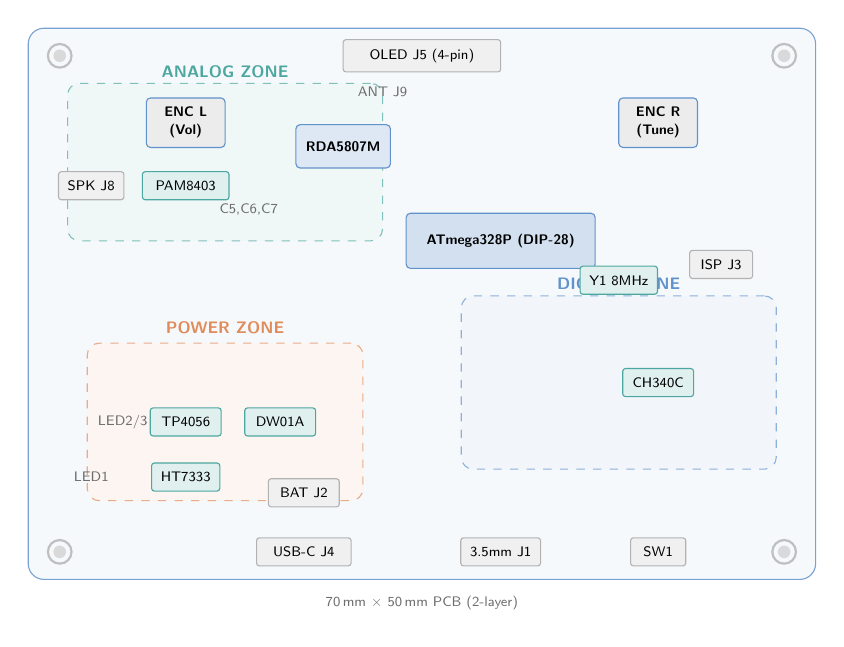
\begin{tikzpicture}[
  board/.style={draw=accentblue!60, fill=accentblue!4, rounded corners=2mm,
                minimum width=10cm, minimum height=7cm},
  zone/.style={draw=#1!50, fill=#1!6, rounded corners=1.5mm, dashed,
               minimum width=4.6cm, minimum height=3.0cm},
  ic/.style={draw=accentblue!70, fill=accentblue!15, rounded corners=1.5pt,
             minimum width=1.3cm, minimum height=0.55cm,
             font=\sffamily\fontsize{5.5}{6.5}\selectfont\bfseries, align=center},
  smd/.style={draw=accentteal!70, fill=accentteal!12, rounded corners=1pt,
              minimum width=0.9cm, minimum height=0.35cm,
              font=\sffamily\fontsize{5}{6}\selectfont, align=center},
  conn/.style={draw=gray!60, fill=gray!12, rounded corners=1pt,
               minimum height=0.35cm,
               font=\sffamily\fontsize{5}{6}\selectfont, align=center},
  lbl/.style={font=\sffamily\fontsize{5}{6}\selectfont, color=codegray},
  zone_lbl/.style={font=\sffamily\fontsize{6}{7}\selectfont\bfseries, color=#1!70},
]
% Board outline
\node[board] (pcb) at (0,0) {};
\node[lbl] at (0,-3.8) {70\,mm $\times$ 50\,mm PCB (2-layer)};

% Zone overlays
\node[zone=accentorange, minimum width=3.5cm, minimum height=2.0cm] at (-2.5,-1.5) {};
\node[zone_lbl=accentorange] at (-2.5,-0.3) {POWER ZONE};

\node[zone=accentblue, minimum width=4.0cm, minimum height=2.2cm] at (2.5,-1.0) {};
\node[zone_lbl=accentblue] at (2.5,0.25) {DIGITAL ZONE};

\node[zone=accentteal, minimum width=4.0cm, minimum height=2.0cm] at (-2.5,1.8) {};
\node[zone_lbl=accentteal] at (-2.5,2.95) {ANALOG ZONE};

% Mounting holes (corners)
\foreach \x/\y in {-4.6/3.15, 4.6/3.15, -4.6/-3.15, 4.6/-3.15} {
  \draw[gray!50, thick] (\x,\y) circle (0.15);
  \fill[gray!30] (\x,\y) circle (0.08);
}

% === SOUTH EDGE (bottom) ===
\node[conn, minimum width=1.2cm] (usbc) at (-1.5,-3.15) {USB-C J4};
\node[conn, minimum width=1.0cm] (jack) at (1.0,-3.15) {3.5mm J1};
\node[conn, minimum width=0.7cm] (sw1)  at (3.0,-3.15) {SW1};

% === NORTH EDGE (top) ===
\node[conn, minimum width=2.0cm] (oled) at (0,3.15) {OLED J5 (4-pin)};

% === ENCODERS (near north) ===
\node[ic, minimum width=1.0cm, fill=gray!15] (enc_l) at (-3.0,2.3) {ENC L\\(Vol)};
\node[ic, minimum width=1.0cm, fill=gray!15] (enc_r) at (3.0,2.3) {ENC R\\(Tune)};

% === CENTRE: ATmega ===
\node[ic, minimum width=2.4cm, minimum height=0.7cm, fill=accentblue!20] (mcu) at (1.0,0.8) {ATmega328P (DIP-28)};

% === POWER ZONE ===
\node[smd] (tp4056) at (-3.0,-1.5) {TP4056};
\node[smd] (dw01) at (-1.8,-1.5) {DW01A};
\node[smd, minimum width=0.7cm] (ht73) at (-3.0,-2.2) {HT7333};
\node[conn, minimum width=0.9cm] (bat) at (-1.5,-2.4) {BAT J2};
\node[lbl] at (-3.8,-1.5) {LED2/3};

% === DIGITAL ZONE ===
\node[smd] (ch340) at (3.0,-1.0) {CH340C};
\node[conn, minimum width=0.8cm] (isp) at (3.8,0.5) {ISP J3};
\node[smd, minimum width=0.6cm] (xtal) at (2.5,0.3) {Y1 8MHz};

% === ANALOG ZONE ===
\node[smd, minimum width=1.1cm] (pam) at (-3.0,1.5) {PAM8403};
\node[ic, minimum width=1.2cm] (rda) at (-1.0,2.0) {RDA5807M};
\node[conn, minimum width=0.7cm] (spk) at (-4.2,1.5) {SPK J8};
\node[lbl] at (-0.5,2.7) {ANT J9};

% C5 coupling caps near PAM
\node[lbl] at (-2.2,1.2) {\tiny C5,C6,C7};

% LED1 near power zone
\node[lbl] at (-4.2,-2.2) {LED1};

\end{tikzpicture}
\end{diagrambox}

\subsection{Noise Reduction and Signal Integrity}

This 2-layer PCB uses a continuous back-copper ground plane and strategic zone separation to minimise noise coupling between the digital MCU, RF radio, and Class-D amplifier.

\begin{enumerate}
    \item \textbf{Ground plane (B.Cu):} Fill the entire back layer with GND copper. This provides a low-impedance return path for all signals and shields the digital traces from the analog audio.
    \item \textbf{Analog/digital separation:} Route analog audio traces (RDA5807M LOUT/ROUT, PAM8403 inputs/outputs, headphone coupling) on the west half of F.Cu. Route digital traces (SPI, UART, encoder signals) on the east half. The ATmega sits at the boundary.
    \item \textbf{PAM8403 ground returns:} Use wide (0.5\,mm+) traces from PAM8403 PGND pins to the nearest ground via. Multiple vias around the PAM8403 reduce ground inductance. The Class-D switching currents must return to ground as locally as possible.
    \item \textbf{R3/R4 mixing resistors:} Place these immediately adjacent to the PAM8403 input pins. Short audio traces reduce noise pickup.
    \item \textbf{Crystal guard ring:} Place ground vias around the 8\,MHz crystal and C3a/C3b. This prevents crystal harmonics from coupling into the RDA5807M receiver.
    \item \textbf{TP4056 / HT7333 input/output capacitors:} Place C9, C10, C12, C15, C17 within 2\,mm of the IC power pins. Short traces between capacitor and pin reduce ESL.
    \item \textbf{Antenna area:} No copper pour or digital traces within 3\,mm of the RDA5807M antenna pad (J9) and the coupling capacitor C8. The antenna trace to the 3.5\,mm jack should be as direct as possible.
    \item \textbf{USB-C / CH340C:} Keep the USB D+/D$-$ traces short and matched-length (under 20\,mm). Place CH340C as close to the USB-C connector as practical.
    \item \textbf{Star-point power distribution:} VBAT fans out from the switch to three destinations: HT7333 IN, PAM8403 PVCC, and R7 divider. Use separate traces (not daisy-chained) to prevent amplifier current spikes from coupling into the LDO.
\end{enumerate}

\begin{warningbox}
\textbf{Keep the antenna area clean.} No ground plane directly under the RDA5807M antenna pad. No high-speed digital traces near the antenna coupling path (C8 $\rightarrow$ jack). This minimizes RF interference.
\end{warningbox}

\subsection{Design Rules Setup}

Edit $\rightarrow$ Board Setup $\rightarrow$ Design Rules:

\begin{longtable}{@{}p{5cm}p{3cm}p{5cm}@{}}
\toprule
\textbf{Parameter} & \textbf{Value} & \textbf{Notes} \\
\midrule
\endhead
Minimum trace width & 0.25\,mm & Default signal traces \\
Power trace width & 0.5--1.0\,mm & +3V3, VBAT, GND \\
Minimum clearance & 0.2\,mm & Between traces \\
Minimum via drill & 0.3\,mm & For signal vias (F.Cu $\leftrightarrow$ B.Cu ground plane) \\
Via annular ring & 0.6\,mm outer diameter & \\
Copper to edge & 0.3\,mm & Keep copper away from board edge \\
\bottomrule
\end{longtable}

\subsection{Routing Traces}

\begin{enumerate}
    \item Press \textbf{X} to start routing a trace
    \item \textbf{Two-layer strategy:} F.Cu for signal traces and component pads. B.Cu is a continuous GND pour. Use vias to connect ground pads to the B.Cu plane.
    \item Route \textbf{power traces first}: VBAT, +3V3 --- use 0.5--1.0\,mm width on F.Cu
    \item Route \textbf{I2C bus}: SDA and SCL --- use 0.3\,mm, short runs
    \item Route \textbf{audio traces}: PAM8403 input/output --- keep in analog zone, away from digital signals
    \item Route \textbf{USB data}: CH340C D+/D$-$ traces matched length, under 20\,mm
    \item Route \textbf{encoder signals}: short runs from edge connectors to MCU
    \item Route all remaining signals
\end{enumerate}

\subsection{Ground Plane Pour}

\begin{enumerate}
    \item Select \textbf{B.Cu} (back copper) layer
    \item Place $\rightarrow$ Add Fill Zone (or press \textbf{Ctrl+Shift+Z})
    \item Draw a rectangle covering the entire board
    \item Assign net: GND
    \item Press \textbf{B} to fill all zones
    \item This creates a continuous ground plane on B.Cu, providing a low-impedance return path and shielding analog from digital. Through-hole GND legs and SMD GND pads connect via stitching vias.
\end{enumerate}

\begin{infobox}
A solid B.Cu ground plane is essential for this mixed SMD/TH design. It provides a low-impedance return path for the Class-D amplifier switching currents, shields the FM radio receiver from MCU digital noise, and ensures the USB-C data lines have proper impedance control.
\end{infobox}

\subsection{Silkscreen}

\begin{enumerate}
    \item Add text labels on F.Silkscreen layer:
    \begin{itemize}[noitemsep]
        \item Project name: ``FM Pocket Radio V3''
        \item Component references (auto-placed by KiCad)
        \item Pin labels near headers: ``SDA'', ``SCL'', ``TX'', ``RX'', ``MISO'', etc.
        \item Polarity markers near electrolytic caps and LEDs
    \end{itemize}
\end{enumerate}

\subsection{Running DRC}

\begin{enumerate}
    \item Inspect $\rightarrow$ Design Rules Checker
    \item Click ``Run DRC''
    \item Fix all errors:
    \begin{itemize}[noitemsep]
        \item Trace clearance violations --- reroute offending traces
        \item Unconnected nets --- add missing traces or vias
        \item Minimum width violations --- widen undersized traces
    \end{itemize}
    \item \textbf{Zero errors required} before generating Gerber files
\end{enumerate}

% ============================================================================
\section{Generating Gerber Files}
\label{sec:gerber}
% ============================================================================

\begin{enumerate}
    \item In PCB Editor: File $\rightarrow$ Fabrication Outputs $\rightarrow$ Gerbers (.gbr)
    \item Set output directory: \texttt{gerbers/}
    \item Select layers to export:
    \begin{itemize}[noitemsep]
        \item F.Cu (front copper --- signal traces and SMD pads)
        \item B.Cu (back copper --- continuous GND ground plane)
        \item F.Silkscreen (component labels, reference designators)
        \item F.Mask (solder mask, top side)
        \item B.Mask (solder mask, bottom side)
        \item F.Paste (solder paste for SMD pads --- needed for reflow/hand soldering)
        \item Edge.Cuts (board outline)
    \end{itemize}
    \item Click ``Plot'' to generate all Gerber files
    \item File $\rightarrow$ Fabrication Outputs $\rightarrow$ Drill Files (.drl)
    \begin{itemize}[noitemsep]
        \item Format: Excellon
        \item Drill origin: Absolute
        \item Click ``Generate Drill File''
    \end{itemize}
    \item \textbf{Verify:} Open Gerber files in KiCad's Gerber Viewer (File $\rightarrow$ Open in new Gerber Viewer). Check each layer visually. Confirm all traces, pads, and board outline are correct.
\end{enumerate}

\subsection{BOM and Pick-and-Place Export (If Shop Does Assembly)}

\begin{enumerate}
    \item File $\rightarrow$ Fabrication Outputs $\rightarrow$ Component Placement (.pos)
    \begin{itemize}[noitemsep]
        \item Format: CSV
        \item Include: all through-hole components
        \item This file tells the shop where to place each component
    \end{itemize}
    \item In Schematic Editor: Tools $\rightarrow$ Edit Symbol Fields $\rightarrow$ Export as CSV
    \begin{itemize}[noitemsep]
        \item This generates the BOM (Bill of Materials)
    \end{itemize}
\end{enumerate}

\subsection{Sending to PCB Shop}

Create a ZIP file containing:
\begin{itemize}[noitemsep]
    \item All Gerber files (.gbr)
    \item Drill file (.drl)
    \item BOM (if assembly needed)
    \item Pick-and-place file (if assembly needed)
    \item A note specifying: \textbf{2-layer (double-sided)}, FR-4, 1.6\,mm thickness, HASL finish, green solder mask; mixed SMD + through-hole. Workshop assembles SMD components (PAM8403, CH340C, TP4056, HT7333, DW01A, FS8205A, USB-C, SMD LEDs).
\end{itemize}

Upload or email to the shop (e.g., LankaPCB, Nilambara, etc.).

% ============================================================================
\section{Enclosure Design --- Laser-Cut Acrylic}
\label{sec:enclosure}
% ============================================================================

\subsection{Concept: Stacked Acrylic Layers}

The enclosure is made by stacking 5--7 layers of laser-cut clear (or tinted) acrylic, held together with M3 bolts through the corners. Each layer has different cutouts.

\begin{diagrambox}
\centering
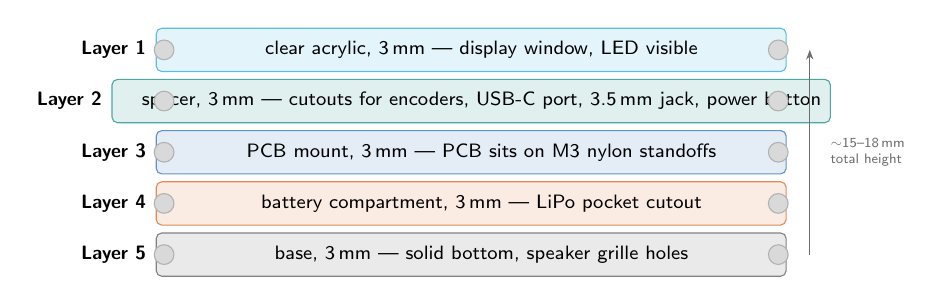
\begin{tikzpicture}[
  layer/.style={draw=#1!70, fill=#1!12, rounded corners=2pt,
                minimum width=8.0cm, minimum height=0.55cm,
                font=\sffamily\scriptsize, align=left},
  bolt/.style={draw=gray!60, fill=gray!30, circle, minimum size=0.25cm, inner sep=0pt},
  lbl/.style={font=\sffamily\tiny, color=codegray, align=left},
  arr/.style={-{Stealth[length=3.5pt]}, thin, color=codegray}
]
% Draw 5 layers stacked
\def\gap{0.65}
\node[layer=accentblue!60!cyan, label=left:{\sffamily\scriptsize\bfseries Layer 1}] (l1)
  at (0,4*\gap) {\quad clear acrylic, 3\,mm --- display window, LED visible};
\node[layer=accentteal, label=left:{\sffamily\scriptsize\bfseries Layer 2}] (l2)
  at (0,3*\gap) {\quad spacer, 3\,mm --- cutouts for encoders, USB-C port, 3.5\,mm jack, power button};
\node[layer=accentblue, label=left:{\sffamily\scriptsize\bfseries Layer 3}] (l3)
  at (0,2*\gap) {\quad PCB mount, 3\,mm --- PCB sits on M3 nylon standoffs};
\node[layer=accentorange, label=left:{\sffamily\scriptsize\bfseries Layer 4}] (l4)
  at (0,1*\gap) {\quad battery compartment, 3\,mm --- LiPo pocket cutout};
\node[layer=gray!60!black, label=left:{\sffamily\scriptsize\bfseries Layer 5}] (l5)
  at (0,0) {\quad base, 3\,mm --- solid bottom, speaker grille holes};

% Corner bolts (left and right)
\foreach \y in {0,\gap,2*\gap,3*\gap,4*\gap} {
  \node[bolt] at (-3.9,\y) {};
  \node[bolt] at  (3.9,\y) {};
}
% Total height label
\draw[arr] (4.3,0) -- (4.3,4*\gap);
\node[lbl, right=4pt] at (4.3, 2*\gap) {$\sim$15--18\,mm\\total height};
\end{tikzpicture}
\end{diagrambox}

\subsection{Layer Drawings (Dimensions in mm)}

All layers are 76\,mm $\times$ 56\,mm (PCB + 3\,mm margin on each side).

\textbf{Layer 1 --- Top (clear acrylic, 3\,mm):}
\begin{itemize}[noitemsep]
    \item 4$\times$ M3 corner holes (3.2\,mm drill)
    \item Display window area: no cutout needed (clear acrylic --- OLED visible through it)
    \item Optional: frosted area over non-display zone for aesthetics
\end{itemize}

\textbf{Layer 2 --- Component Clearance Spacer (3\,mm):}
\begin{itemize}[noitemsep]
    \item 4$\times$ M3 corner holes
    \item Large rectangular cutout in center (for OLED, encoders, tall components)
    \item Side cutouts for: encoder shafts, USB-C port, 3.5\,mm jack, power button
\end{itemize}

\textbf{Layer 3 --- PCB Mount (3\,mm):}
\begin{itemize}[noitemsep]
    \item 4$\times$ M3 corner holes (outer)
    \item 4$\times$ M3 holes matching PCB mount holes (for standoffs)
    \item Side cutouts for: USB-C port, 3.5\,mm jack, power button
\end{itemize}

\textbf{Layer 4 --- Battery Space (3--6\,mm, may use 2 layers):}
\begin{itemize}[noitemsep]
    \item Large cutout for LiPo battery ($\sim$50\,mm $\times$ 35\,mm $\times$ 5\,mm)
    \item Side cutout for battery wires
\end{itemize}

\textbf{Layer 5 --- Bottom (3\,mm, opaque or clear):}
\begin{itemize}[noitemsep]
    \item 4$\times$ M3 corner holes
    \item Speaker grille: array of 2\,mm holes in a circular pattern ($\sim$30\,mm diameter) centered under speaker
    \item Rubber feet mounting points
\end{itemize}

\subsection{Design in Fusion 360}

\begin{enumerate}
    \item Export PCB as STEP: In KiCad PCB Editor, File $\rightarrow$ Export $\rightarrow$ STEP
    \item Open Fusion 360
    \item Insert $\rightarrow$ Insert Mesh/STEP $\rightarrow$ import the PCB STEP file
    \item Create each acrylic layer as a sketch + extrude (3\,mm each)
    \item Add cutouts using the PCB model as reference for component positions
    \item Export each layer as DXF: right-click face $\rightarrow$ Save as DXF
    \item Send DXF files to laser cutting shop
\end{enumerate}

\begin{infobox}
\textbf{Alternative to Fusion 360:} You can design the 2D layer profiles in \textbf{Inkscape} (free) or \textbf{LibreCAD} (free). Draw each layer as a 2D outline with cutouts, export as DXF or SVG. This is faster if you're not comfortable with Fusion 360.
\end{infobox}

\subsection{Assembly}

\begin{enumerate}
    \item Stack layers bottom to top: Layer 5 $\rightarrow$ 4 $\rightarrow$ 3 $\rightarrow$ 2 $\rightarrow$ 1
    \item Insert M3$\times$20mm screws from bottom up through all 4 corner holes
    \item Place nylon standoffs between Layer 3 and PCB
    \item Mount PCB on standoffs
    \item Tighten M3 nuts on top (or use acorn nuts for clean look)
    \item Battery sits in Layer 4 cutout, connected to PCB via JST connector
\end{enumerate}

% ============================================================================
\section{Firmware}
\label{sec:firmware}
% ============================================================================

\subsection{Arduino IDE Setup}

\begin{enumerate}
    \item Open Arduino IDE (1.8.x or 2.x)
    \item Tools $\rightarrow$ Board $\rightarrow$ ``\textbf{Arduino Pro or Pro Mini}''
    \item Tools $\rightarrow$ Processor $\rightarrow$ ``\textbf{ATmega328P (3.3V, 8 MHz)}''
    \item Tools $\rightarrow$ Programmer $\rightarrow$ ``Arduino as ISP'' (for bootloader)
\end{enumerate}

\subsection{Required Libraries}

Install via Sketch $\rightarrow$ Include Library $\rightarrow$ Manage Libraries:
\begin{itemize}[noitemsep]
    \item \textbf{U8g2} by oliver (for SSD1306 OLED display)
    \item \textbf{Wire} (built-in, for I2C)
    \item \textbf{EEPROM} (built-in, replaces ESP32 Preferences/NVS)
\end{itemize}

\subsection{Complete Firmware Source Code}

\begin{infobox}
This firmware was designed with UI/UX prototyped first as a Python/Pillow simulation (see project repo). The three ``premium'' UX behaviours translated from the simulation:\begin{itemize}[noitemsep]
\item \textbf{Station name scrolling} --- long names pan left/right automatically
\item \textbf{Volume slot-machine tween} --- old number slides out, new number slides in
\item \textbf{Tactile flash} --- white screen for one frame on button press, mimics physical ``clack''
\end{itemize}
\end{infobox}

\begin{lstlisting}[language=C++, caption={FM Pocket Radio --- ATmega328P Firmware Rev 2 (fm\_pocket\_radio.ino)}]
/*
 * FM Pocket Radio - ATmega328P Firmware (Rev 2 - Premium UX)
 * Board: "Arduino Pro or Pro Mini"
 * Processor: "ATmega328P (3.3V, 8 MHz)"
 * Programming: USB-C (on-board CH340C) --- same port as charging
 *
 * UX features ported from Python/Pillow simulation:
 *   - Station name auto-scroll for long names
 *   - Volume tween (slot-machine reel animation)
 *   - Tactile flash on button press
 */

#include <Wire.h>
#include <U8g2lib.h>
#include <EEPROM.h>

// ==================== PIN DEFINITIONS ====================
#define PIN_ENC_R_CLK  2   // Right encoder CLK (INT0 hardware interrupt)
#define PIN_ENC_L_CLK  3   // Left encoder CLK  (INT1 hardware interrupt)
#define PIN_ENC_R_DT   4   // Right encoder DT
#define PIN_ENC_L_DT   5   // Left encoder DT
#define PIN_ENC_R_SW   6   // Right encoder switch -> Seek UP
#define PIN_ENC_L_SW   7   // Left encoder switch  -> Seek DOWN
#define PIN_HP_DET     8   // Headphone detect (LOW = plugged in)
#define PIN_AMP_EN     9   // PAM8403 ~SHDN: HIGH = amplifier on, LOW = mute
#define PIN_BAT_ADC    A0  // Battery voltage divider midpoint

// ==================== RDA5807M ====================
#define RDA_ADDR    0x10
#define FREQ_MIN_10 875
#define FREQ_MAX_10 1080

U8G2_SSD1306_128X64_NONAME_F_HW_I2C oled(U8G2_R0, U8X8_PIN_NONE);
static uint16_t reg[8];

// ==================== RUNTIME STATE ====================
volatile int8_t encRDelta = 0;
volatile int8_t encLDelta = 0;
uint16_t freq10     = 939;
uint8_t  volume     = 8;
int      sigLevel   = 0;
int      batPercent = 100;
bool     hpPlugged  = false;
uint32_t lastChange = 0;
bool     needSave   = false;
uint32_t lastBtnR   = 0, lastBtnL = 0;
uint32_t lastDisp   = 0, bootTime = 0;
bool     booting    = true;

#define EE_MAGIC_ADDR 0
#define EE_FREQ_ADDR  1
#define EE_VOL_ADDR   3
#define EE_MAGIC_VAL  0xAA

// ==================== UX STATE ====================
bool     flashPending = false;   // tactile flash: white 1 frame
uint8_t  oldVolume    = 8;
int8_t   volAnimY     = 11;      // 11=settled, 0-10=animating

enum ScrollState {
  SCR_IDLE, SCR_WAIT_START, SCR_FWD, SCR_PAUSE_END,
  SCR_BACK, SCR_PAUSE_START
};
ScrollState scrollState = SCR_WAIT_START;
int16_t     scrollX     = 0;
uint32_t    scrollTimer = 0;
uint16_t    prevFreq10  = 0;

// ==================== STATION DATABASE (PROGMEM) ====================
typedef struct { uint16_t freq10; char name[16]; } Station;
const Station PROGMEM stations[] = {
  { 876,"Lite FM"        },{ 883,"E FM"           },
  { 886,"Singha FM"      },{ 891,"Isira TNL FM"   },
  { 896,"City FM"        },{ 904,"Vettri FM"      },
  { 909,"Shaa FM"        },{ 914,"Alai FM"        },
  { 922,"FM Derana"      },{ 927,"Y FM"           },
  { 930,"Gold FM"        },{ 935,"Lakhanda"       },
  { 948,"Neth FM"        },{ 956,"Rhythm FM"      },
  { 961,"Hiru FM"        },{ 966,"Kiriula FM"     },
  { 969,"Kiss FM"        },{ 971,"Real Radio"     },
  { 974,"Radio Sri Lanka"},{ 982,"Siyatha FM"     },
  { 987,"Sun FM"         },{ 992,"TNL Rocks"      },
  { 995,"Red FM"         },{1000,"Shree FM"       },
  {1005,"Ran FM"         },{1008,"Yes FM"         },
  {1018,"Seth FM"        },{1021,"Tamil NS"       },
  {1026,"Vasantham"      },{1034,"Sooriyan FM"    },
  {1039,"Shakthi FM"     },{1044,"Rangiri SL"     },
  {1047,"Thendral"       },{1052,"Lakviru FM"     },
  {1060,"Lak FM"         },{1065,"Sirasa FM"      },
  {1070,"V FM"           },{1073,"Kandurata"      },
};
const uint8_t NUM_STATIONS = sizeof(stations)/sizeof(Station);

void getStationName(uint16_t f, char* buf, uint8_t len) {
  Station s;
  for (uint8_t i = 0; i < NUM_STATIONS; i++) {
    memcpy_P(&s, &stations[i], sizeof(Station));
    int d = (int)f - (int)s.freq10;
    if (d >= -1 && d <= 1) {
      strncpy(buf, s.name, len-1); buf[len-1]='\0'; return;
    }
  }
  strncpy(buf, "MANUAL TUNE", len-1); buf[len-1]='\0';
}

// ==================== RDA5807M DRIVER ====================
static void rdaWrite() {
  Wire.beginTransmission(RDA_ADDR);
  for (uint8_t r=2; r<=7; r++) {
    Wire.write((uint8_t)(reg[r]>>8));
    Wire.write((uint8_t)(reg[r]&0xFF));
  }
  Wire.endTransmission();
}
static uint16_t rdaRead0A() {
  Wire.requestFrom((uint8_t)RDA_ADDR, (uint8_t)4);
  uint8_t a=Wire.read(), b=Wire.read();
  uint8_t c=Wire.read(); Wire.read();
  sigLevel = constrain((c>>1)/4, 0, 15);
  return ((uint16_t)a<<8)|b;
}
static void rdaInit() {
  reg[2]=0xC001; reg[3]=0; reg[4]=0x0A00;
  reg[5]=(0x88A0&0xFFF0)|(volume&0x0F);
  reg[6]=0; reg[7]=0;
  rdaWrite(); delay(200);
}
static void rdaTune(uint16_t f) {
  uint16_t ch = f-870;
  reg[3]=(ch<<6)|(1u<<4); rdaWrite(); delay(80);
  reg[3]&=~(1u<<4);       rdaWrite();
}
static void rdaSetVol(uint8_t v) {
  v=constrain(v,0,15);
  reg[5]=(reg[5]&0xFFF0)|v; rdaWrite();
}
static bool rdaSeek(bool up) {
  if (up) reg[2]|=(1u<<9); else reg[2]&=~(1u<<9);
  reg[2]|=(1u<<8); rdaWrite(); delay(200);
  uint16_t st=0;
  for (uint8_t i=0; i<80; i++) {
    st=rdaRead0A(); if (st&(1u<<14)) break; delay(50);
  }
  reg[2]&=~(1u<<8); rdaWrite(); delay(50); rdaRead0A();
  if (st&(1u<<13)) return false;
  freq10=constrain(870+(st&0x03FF), FREQ_MIN_10, FREQ_MAX_10);
  return true;
}

// ==================== ENCODER ISRs ====================
void isrEncR() { encRDelta += digitalRead(PIN_ENC_R_DT)?-1:1; }
void isrEncL() { encLDelta += digitalRead(PIN_ENC_L_DT)?-1:1; }

// ==================== BATTERY ====================
int readBattery() {
  long s=0;
  for (uint8_t i=0; i<16; i++) s+=analogRead(PIN_BAT_ADC);
  float v=(s/16.0)*(3.3/1023.0)*2.0;
  if (v>=4.20) return 100; if (v>=4.10) return 90;
  if (v>=4.00) return 80;  if (v>=3.90) return 60;
  if (v>=3.80) return 40;  if (v>=3.70) return 30;
  if (v>=3.60) return 15;  return 0;
}

// ==================== EEPROM ====================
void loadSettings() {
  if (EEPROM.read(EE_MAGIC_ADDR)==EE_MAGIC_VAL) {
    uint8_t lo=EEPROM.read(EE_FREQ_ADDR);
    uint8_t hi=EEPROM.read(EE_FREQ_ADDR+1);
    freq10=constrain(((uint16_t)hi<<8)|lo, FREQ_MIN_10,FREQ_MAX_10);
    volume=constrain(EEPROM.read(EE_VOL_ADDR), 0, 15);
  }
}
void saveSettings() {
  EEPROM.update(EE_MAGIC_ADDR, EE_MAGIC_VAL);
  EEPROM.update(EE_FREQ_ADDR,   (uint8_t)(freq10&0xFF));
  EEPROM.update(EE_FREQ_ADDR+1, (uint8_t)(freq10>>8));
  EEPROM.update(EE_VOL_ADDR, volume);
}

// ==================== DISPLAY ====================
static uint8_t eqH[20];
static uint16_t rng = 0xACE1;  // LFSR seed
static void advanceEq() {
  for (uint8_t i=0; i<20; i++) {
    rng^=rng<<7; rng^=rng>>9; rng^=rng<<8;
    eqH[i] = 2+(rng&0x07);
  }
}

void drawBoot() {
  oled.clearBuffer();
  oled.setFont(u8g2_font_ncenB14_tr);
  uint16_t w=oled.getStrWidth("FM RADIO");
  oled.drawStr((128-w)/2, 28, "FM RADIO");
  oled.setFont(u8g2_font_ncenB10_tr);
  w=oled.getStrWidth("EE2050");
  oled.drawStr((128-w)/2, 52, "EE2050");
  oled.sendBuffer();
}

void drawMain() {
  oled.clearBuffer();
  oled.setFont(u8g2_font_5x7_tr);

  // Signal bars (top-left, 4 bars)
  int bars=sigLevel/4;
  for (int i=0; i<4; i++) {
    uint8_t h=3+i*2, bx=1+i*4, by=10-h;
    if (i<bars) oled.drawBox(bx,by,3,h);
    else        oled.drawFrame(bx,by,3,h);
  }

  // Battery icon (top-right)
  char tmp[8]; snprintf(tmp,sizeof(tmp),"%d%%",batPercent);
  uint8_t tw=oled.getStrWidth(tmp), tx=128-tw-2;
  oled.drawStr(tx, 9, tmp);
  oled.drawFrame(tx-15, 1, 13, 8);
  oled.drawBox(tx-2, 3, 2, 4);
  int bf=(batPercent*11)/100;
  if (bf>0) oled.drawBox(tx-14, 2, bf, 6);

  // Speaker icon (center-top)
  uint8_t sx=53;
  oled.drawBox(sx, 3, 3, 5);
  oled.drawLine(sx+3,2,sx+7,0); oled.drawLine(sx+3,7,sx+7,10);
  oled.drawLine(sx+7,0,sx+7,10);
  if (volume> 0) oled.drawLine(sx+ 9,4,sx+ 9,7);
  if (volume> 5) oled.drawLine(sx+11,3,sx+11,8);
  if (volume>10) oled.drawLine(sx+13,2,sx+13,9);

  // Volume -- slot-machine tween (ported from Python sim)
  uint8_t vx=sx+15;
  if (volAnimY<11) {
    int8_t oy=9-volAnimY, ny=9-volAnimY+11;
    char olds[4], news[4];
    snprintf(olds,4,"%d",oldVolume); snprintf(news,4,"%d",volume);
    if (oy>=0 && oy<=10) oled.drawStr(vx, oy, olds);
    if (ny>=0 && ny<=10) oled.drawStr(vx, ny, news);
  } else {
    snprintf(tmp,sizeof(tmp),"%d",volume);
    oled.drawStr(vx, 9, tmp);
  }

  // Frequency (large, centred)
  oled.setFont(u8g2_font_ncenB14_tr);
  snprintf(tmp,sizeof(tmp),"%d.%d",freq10/10,freq10%10);
  uint16_t fw=oled.getStrWidth(tmp);
  oled.drawStr((128-fw)/2, 26, tmp);
  oled.setFont(u8g2_font_5x7_tr);
  oled.drawStr((128-fw)/2+fw+2, 17, "MHz");

  // Station name with SCROLL (ported from Python sim)
  oled.setFont(u8g2_font_7x14B_tr);
  char stn[16]; getStationName(freq10, stn, sizeof(stn));
  uint16_t nw=oled.getStrWidth(stn);
  if (nw<=126) oled.drawStr((128-nw)/2, 40, stn);
  else         oled.drawStr(4-scrollX, 40, stn);

  // Equalizer bars (bottom)
  oled.setFont(NULL);
  for (uint8_t i=0; i<20; i++)
    oled.drawBox(4+i*6, 63-eqH[i], 5, eqH[i]);

  // Status line (HP + ST/MO)
  oled.setFont(u8g2_font_5x7_tr);
  if (hpPlugged) oled.drawStr(0, 63, "HP");
  uint16_t st=rdaRead0A();
  oled.drawStr(12, 63, (st&(1u<<10))?"ST":"MO");

  oled.sendBuffer();
}

void drawSeek() {
  oled.clearBuffer();
  oled.setFont(u8g2_font_7x14B_tr);
  uint16_t w=oled.getStrWidth("Seeking...");
  oled.drawStr((128-w)/2, 36, "Seeking...");
  static uint8_t scanX=0; scanX=(scanX+4)%108;
  oled.drawLine(10,50,118,50);
  oled.drawLine(10+scanX,46,10+scanX,54);
  oled.sendBuffer();
}

// ==================== SETUP ====================
void setup() {
  pinMode(PIN_ENC_R_CLK, INPUT_PULLUP);
  pinMode(PIN_ENC_L_CLK, INPUT_PULLUP);
  pinMode(PIN_ENC_R_DT,  INPUT_PULLUP);
  pinMode(PIN_ENC_L_DT,  INPUT_PULLUP);
  pinMode(PIN_ENC_R_SW,  INPUT_PULLUP);
  pinMode(PIN_ENC_L_SW,  INPUT_PULLUP);
  pinMode(PIN_HP_DET,    INPUT_PULLUP);
  pinMode(PIN_AMP_EN,    OUTPUT);
  digitalWrite(PIN_AMP_EN, LOW);

  loadSettings(); oldVolume=volume;
  Wire.begin(); oled.begin();
  drawBoot(); bootTime=millis(); booting=true;
  rdaInit(); rdaSetVol(0); rdaTune(freq10);  // start at vol 0 to suppress boot pop
  prevFreq10=freq10; advanceEq();

  attachInterrupt(digitalPinToInterrupt(PIN_ENC_R_CLK),isrEncR,FALLING);
  attachInterrupt(digitalPinToInterrupt(PIN_ENC_L_CLK),isrEncL,FALLING);
  delay(500);  // let amp + DAC settle before enabling speaker
  hpPlugged=!digitalRead(PIN_HP_DET);
  digitalWrite(PIN_AMP_EN, hpPlugged?LOW:HIGH);

  // Ramp volume from 0 to saved value to prevent pop
  for (uint8_t v = 1; v <= volume; v++) {
    rdaSetVol(v);
    delay(30);
  }
}

// ==================== MAIN LOOP ====================
void loop() {
  uint32_t now=millis();
  if (booting && (now-bootTime>2000)) booting=false;

  // Right encoder: tuning (atomic read of ISR variable)
  noInterrupts();
  int8_t rD=encRDelta; encRDelta=0;
  interrupts();
  if (rD && !booting) {
    int16_t f=(int16_t)freq10+rD;
    if (f>FREQ_MAX_10) f=FREQ_MIN_10;
    if (f<FREQ_MIN_10) f=FREQ_MAX_10;
    freq10=f; rdaTune(freq10);
    lastChange=now; needSave=true;
  }

  // Left encoder: volume (atomic read of ISR variable)
  noInterrupts();
  int8_t lD=encLDelta; encLDelta=0;
  interrupts();
  if (lD && !booting) {
    uint8_t nv=constrain((int)volume+lD, 0, 15);
    if (nv!=volume) {
      oldVolume=volume; volume=nv;
      volAnimY=0;
      rdaSetVol(volume);
      lastChange=now; needSave=true;
    }
  }

  // Right button: Seek UP + tactile flash
  if (!digitalRead(PIN_ENC_R_SW) && (now-lastBtnR>300)) {
    lastBtnR=now; flashPending=true;
    drawSeek(); rdaSeek(true);
    scrollState=SCR_WAIT_START; scrollX=0;
    lastChange=now; needSave=true;
  }

  // Left button: Seek DOWN + tactile flash
  if (!digitalRead(PIN_ENC_L_SW) && (now-lastBtnL>300)) {
    lastBtnL=now; flashPending=true;
    drawSeek(); rdaSeek(false);
    scrollState=SCR_WAIT_START; scrollX=0;
    lastChange=now; needSave=true;
  }

  // Reset scroll on frequency change
  if (freq10!=prevFreq10) {
    prevFreq10=freq10;
    scrollState=SCR_WAIT_START; scrollX=0; scrollTimer=now;
  }

  // Headphone detect
  bool hp=!digitalRead(PIN_HP_DET);
  if (hp!=hpPlugged) {
    hpPlugged=hp;
    digitalWrite(PIN_AMP_EN, hpPlugged?LOW:HIGH);
  }

  // Battery every 5 s
  static uint32_t lastBat=0;
  if (now-lastBat>5000) { lastBat=now; batPercent=readBattery(); }

  // EEPROM save (2 s debounce)
  if (needSave && (now-lastChange>2000)) { saveSettings(); needSave=false; }

  // Display at 100 ms
  if (now-lastDisp<100) return;
  lastDisp=now;

  // Advance animations
  if (volAnimY<11) volAnimY+=2;
  advanceEq();

  // Scroll state machine
  char stn[16]; getStationName(freq10, stn, sizeof(stn));
  oled.setFont(u8g2_font_7x14B_tr);
  uint16_t nw=oled.getStrWidth(stn);
  bool needsScroll=(nw>126);
  if (needsScroll) {
    switch (scrollState) {
      case SCR_WAIT_START:
        if (now-scrollTimer>1500) scrollState=SCR_FWD; break;
      case SCR_IDLE:
        scrollState=SCR_WAIT_START; scrollTimer=now; break;
      case SCR_FWD:
        scrollX+=2;
        if (scrollX>=(int16_t)(nw-120)) {
          scrollX=nw-120;
          scrollState=SCR_PAUSE_END; scrollTimer=now;
        } break;
      case SCR_PAUSE_END:
        if (now-scrollTimer>1500) scrollState=SCR_BACK; break;
      case SCR_BACK:
        scrollX-=2;
        if (scrollX<=0) {
          scrollX=0;
          scrollState=SCR_PAUSE_START; scrollTimer=now;
        } break;
      case SCR_PAUSE_START:
        if (now-scrollTimer>2000) scrollState=SCR_FWD; break;
    }
  } else {
    scrollX=0; scrollState=SCR_IDLE;
  }

  // Render frame
  if (flashPending) {
    flashPending=false;
    oled.clearBuffer();
    oled.setDrawColor(1);
    oled.drawBox(0,0,128,64);
    oled.sendBuffer();
  } else if (booting) {
    drawBoot();
  } else {
    drawMain();
  }
}
\end{lstlisting}

% ============================================================================
\section{Programming the ATmega328P}
\label{sec:programming}
% ============================================================================

\subsection{Step 1: Burn Bootloader (One-Time Only)}

You need an Arduino UNO to act as an ISP programmer.

\begin{enumerate}
    \item \textbf{Prepare Arduino UNO as ISP:}
    \begin{itemize}[noitemsep]
        \item Connect Arduino UNO to your PC via USB
        \item In Arduino IDE: File $\rightarrow$ Examples $\rightarrow$ 11.ArduinoISP $\rightarrow$ ArduinoISP
        \item Tools $\rightarrow$ Board $\rightarrow$ ``Arduino Uno''
        \item Click Upload (this programs the UNO as an ISP programmer)
    \end{itemize}
    
    \item \textbf{Connect UNO to your PCB's ISP header:}
    
    \begin{tabular}{ll}
    \toprule
    \textbf{Arduino UNO Pin} & \textbf{PCB ISP Header Pin} \\
    \midrule
    D10 & RESET (pin 5) \\
    D11 (MOSI) & MOSI (pin 4) \\
    D12 (MISO) & MISO (pin 1) \\
    D13 (SCK) & SCK (pin 3) \\
    5V or 3.3V & VCC (pin 2) --- \textbf{USE 3.3V!} \\
    GND & GND (pin 6) \\
    \bottomrule
    \end{tabular}
    
    \begin{warningbox}
    \textbf{Use the UNO's 3.3V pin, NOT 5V}, to power the PCB during programming. The RDA5807M and other 3.3V components are connected to the same power bus. \textbf{Note:} The UNO's 3.3V pin supplies only $\sim$50\,mA (via the FTDI/CH340 regulator). This is sufficient for bare ATmega + passive components during bootloader burn, but \textbf{not} for the full radio (OLED + RDA + PAM8403). For full-system ISP programming, use the radio's own battery: turn SW1 ON, then connect only MISO/MOSI/SCK/RESET/GND from the UNO (no VCC wire).
    \end{warningbox}
    
    \item \textbf{Burn the bootloader:}
    \begin{itemize}[noitemsep]
        \item Tools $\rightarrow$ Board $\rightarrow$ ``Arduino Pro or Pro Mini''
        \item Tools $\rightarrow$ Processor $\rightarrow$ ``ATmega328P (3.3V, 8 MHz)''
        \item Tools $\rightarrow$ Programmer $\rightarrow$ ``Arduino as ISP''
        \item Tools $\rightarrow$ Burn Bootloader
        \item Wait for ``Done burning bootloader'' message
    \end{itemize}
\end{enumerate}

\subsection{Step 2: Upload Firmware (Repeatable)}

Firmware is uploaded via the \textbf{USB-C port} (J4). The on-board CH340C converts USB to serial automatically.

\begin{enumerate}
    \item \textbf{Plug a USB-C cable} from your PC into J4 on the PCB.
    
    \begin{dangerbox}
    \textbf{The radio must be switched ON (SW1) before uploading firmware!} The CH340C and ATmega are powered from the +3V3 rail via the HT7333 LDO, which is downstream of the power switch SW1. If SW1 is OFF, the CH340C has no power and the PC will not detect a COM port. Always turn the radio ON first, then plug in USB-C.
    \end{dangerbox}
    
    \item \textbf{In Arduino IDE:}
    \begin{itemize}[noitemsep]
        \item Tools $\rightarrow$ Board $\rightarrow$ ``Arduino Pro or Pro Mini''
        \item Tools $\rightarrow$ Processor $\rightarrow$ ``ATmega328P (3.3V, 8 MHz)''
        \item Tools $\rightarrow$ Port $\rightarrow$ (select the CH340 COM port, e.g., COM5)
        \item Click Upload
    \end{itemize}
    
    \item The 100\,nF cap (C14) between CH340C DTR\# and RESET auto-resets the ATmega into bootloader mode. No buttons needed.
    
    \item Upload completes in $\sim$5 seconds. Unplug the USB-C cable (or leave it in to charge simultaneously).
\end{enumerate}

\begin{infobox}
\textbf{Charging and programming share the same USB-C port.} While uploading firmware, the TP4056 also receives 5\,V VBUS and charges the battery simultaneously. This is safe --- the TP4056 and CH340C share VBUS/GND but have independent data paths.
\end{infobox}

\begin{warningbox}
\textbf{Charge-while-use caveat:} The radio \textbf{can} operate while USB-C is plugged in (battery charges while radio plays). However, the TP4056's charge termination may be delayed or inaccurate under load, and the battery may not reach a true 4.2\,V endpoint. For the fastest, most reliable charge, \textbf{turn the radio OFF} (SW1) while charging.
\end{warningbox}

\subsection{Troubleshooting Programming}

\begin{longtable}{@{}p{5cm}p{8cm}@{}}
\toprule
\textbf{Problem} & \textbf{Solution} \\
\midrule
\endhead
``avrdude: stk500\_recv(): programmer is not responding'' & Check wiring. Ensure MISO/MOSI/SCK/RESET are correct. Ensure UNO has ArduinoISP sketch uploaded. \\
``avrdude: Yikes! Invalid device signature'' & Wrong board selected, or chip is not powered. Check 3.3V supply. \\
USB-C not detected as COM port & Install CH340 driver from WCH website. Windows 10/11 usually auto-detects. Try a different USB-C cable (data-capable, not charge-only). \textbf{Ensure the radio is switched ON (SW1)} --- the CH340C is powered via the +3V3 rail through SW1. \\
Upload via USB-C not working & Bootloader not burned. Re-burn via ISP. Verify C14 (100\,nF) connects CH340C DTR\# to RESET. \\
Upload times out & TX/RX crossed? CH340C TXD goes to ATmega RX (D0); CH340C RXD goes to ATmega TX (D1). \\
\bottomrule
\end{longtable}

% ============================================================================
\section{Assembly Guide}
\label{sec:assembly}
% ============================================================================

\subsection{If PCB Shop Pre-Solders}

This design uses a \textbf{mix of SMD and through-hole}. The university workshop solders the SMD components; you complete the through-hole parts and modules at home.

\textbf{Workshop solders (SMD --- requires hot air station or reflow):}
\begin{enumerate}[noitemsep]
    \item PAM8403 (SOP-16) --- Class-D amplifier
    \item CH340C (SOP-16) --- USB-to-serial
    \item TP4056 (SOP-8) --- LiPo charger
    \item HT7333 (SOT-89) --- 3.3\,V LDO
    \item DW01A (SOT-23) + FS8205A (SOT-23-6) --- battery protection
    \item USB-C receptacle (SMD)
    \item LED2 (red, 0805) --- CHG indicator
    \item LED3 (green, 0805) --- STDBY indicator
\end{enumerate}

\textbf{You solder at home (through-hole):}
\begin{enumerate}[noitemsep]
    \item ATmega328P-PU (DIP-28) --- in socket or direct solder
    \item Crystal Y1 + load caps C3a/C3b (22\,pF)
    \item All resistors R1--R8, R14 (axial through-hole)
    \item Bypass caps C1, C2, C4 (ceramic disc through-hole)
    \item Electrolytic caps C6, C7, C9, C10, C16 --- observe polarity!
    \item Small ceramic cap C8 (100\,pF, antenna coupling)
    \item Power LED (LED1, 3mm red) --- observe polarity!
    \item ISP header J3
    \item Pin headers: OLED J5, Encoders J6
    \item JST battery connector J2
    \item 3.5\,mm audio jack J1 (PJ-320A)
    \item Speaker terminal J8
    \item Latching push button SW1
    \item Antenna pad J9
\end{enumerate}

\textbf{You plug in (no soldering required):}
\begin{enumerate}[noitemsep]
    \item OLED module into J5 header (check GND/VCC/SCL/SDA orientation)
    \item RDA5807M module (solder flat castellated pads to PCB footprint)
    \item LiPo battery JST PH connector to J2
    \item USB-C cable for charging and programming (then unplug)
\end{enumerate}

\subsection{If Hand-Soldering Everything}

\textbf{Order of soldering} (lowest profile first, modules last):

\begin{enumerate}
    \item Resistors R1--R8, R14 (lay flat, axial through-hole)
    \item Low-profile through-hole: ceramic capacitors, crystal
    \item IC socket (if using DIP-28 ATmega328P --- \textbf{do not insert chip yet})
    \item Taller components: electrolytic capacitors (observe polarity!), LEDs (observe polarity!)
    \item Connectors: 3.5\,mm jack, JST battery connector, speaker pads
    \item Push button (SW1)
    \item Last: insert ATmega328P into socket (align notch/pin 1)
\end{enumerate}

\subsection{Module Installation}

\begin{enumerate}
    \item \textbf{RDA5807M module:} Solder directly to PCB footprint (castellated pads at 1.27\,mm pitch). Use flux and fine-tipped iron. Or solder header pins to the module and plug into matching PCB headers.
    \item \textbf{SSD1306 OLED:} Plug into 4-pin header J5. Check pin order: GND, VCC, SCL, SDA.
    
    \begin{warningbox}
    \textbf{OLED module pin order varies by manufacturer!} Some modules use GND--VCC--SCL--SDA, others use VCC--GND--SCL--SDA or even SDA--SCL--VCC--GND. \textbf{Always verify your specific module's pin order} before plugging in. Reversing VCC and GND \textbf{will damage the OLED.} Label J5 on the PCB silkscreen with the expected pin order.
    \end{warningbox}
    \item \textbf{Encoders:} Connect via 5-pin headers (J6). Route wires to enclosure mounting holes.
\end{enumerate}

\subsection{Final Assembly}

\begin{enumerate}
    \item Plug in battery (JST connector)
    \item Do NOT close the enclosure yet
    \item Proceed to testing (Section~\ref{sec:testing})
    \item After all tests pass, mount PCB in enclosure
\end{enumerate}

% ============================================================================
\section{Testing \& Verification}
\label{sec:testing}
% ============================================================================

Follow these tests in order. Do not skip steps.

\subsection{Test 1: Visual Inspection}

\begin{itemize}
    \item[$\square$] Check all solder joints for bridges (shorts) under magnification
    \item[$\square$] Verify ATmega328P orientation (notch at pin 1)
    \item[$\square$] Verify electrolytic cap polarity (stripe = negative)
    \item[$\square$] Verify LED polarity (flat side = cathode)
    \item[$\square$] Verify SMD solder joints: TP4056, CH340C, PAM8403, HT7333, DW01A, USB-C connector (no bridges, no cold joints)
\end{itemize}

\subsection{Test 2: Power Supply (Before Inserting ICs)}

If using a DIP socket, do this test \textbf{without} the ATmega328P inserted.

\begin{enumerate}
    \item Connect battery via JST connector
    \item Press power switch ON
    \item[$\square$] Measure VBAT: should be 3.0--4.2\,V
    \item[$\square$] Measure +3V3 rail: should be 3.3\,V ($\pm$0.1\,V)
    \item[$\square$] Power LED lights up
    \item[$\square$] No components getting hot
    \item Press power switch OFF
    \item[$\square$] All voltages drop to 0\,V
\end{enumerate}

\subsection{Test 3: TP4056 Charging via USB-C}

\begin{enumerate}
    \item Plug a USB-C cable from a 5\,V charger (or PC) into J4
    \item[$\square$] Red CHG LED (LED2 on PCB) lights up --- battery is charging
    \item[$\square$] Measure BAT pad: should be charging voltage (3.0--4.2\,V rising)
    \item Wait until green STDBY LED (LED3 on PCB) lights up --- battery full
    \item[$\square$] No components getting excessively hot (warm is OK, hot is not)
\end{enumerate}

\subsection{Test 4: MCU Boot}

\begin{enumerate}
    \item Insert ATmega328P (if DIP socket)
    \item Burn bootloader (Section~\ref{sec:programming})
    \item Upload firmware
    \item Power on
    \item[$\square$] Boot screen appears on OLED (``FM RADIO'', ``EE2050'') for 2 seconds
    \item[$\square$] Main screen appears after boot
\end{enumerate}

\subsection{Test 5: I2C Scan}

Upload a basic I2C scanner sketch first (before the radio firmware):

\begin{lstlisting}[language=C++,numbers=none]
#include <Wire.h>
void setup() {
  Wire.begin();
  Serial.begin(9600);
  for (byte a = 1; a < 127; a++) {
    Wire.beginTransmission(a);
    if (Wire.endTransmission() == 0) {
      Serial.print("Found: 0x");
      Serial.println(a, HEX);
    }
  }
}
void loop() {}
\end{lstlisting}

\begin{itemize}
    \item[$\square$] Serial output shows: \texttt{Found: 0x10} (RDA5807M)
    \item[$\square$] Serial output shows: \texttt{Found: 0x3C} (SSD1306)
\end{itemize}

\begin{infobox}
\textbf{RDA5807M address note:} Most RDA5807M modules respond at \texttt{0x10} (sequential write mode). Some modules may also appear at \texttt{0x11} (random-access mode). If you see \texttt{0x11} instead of (or in addition to) \texttt{0x10}, the module is working correctly --- the firmware uses the 0x10 address for sequential register writes.
\end{infobox}

\subsection{Test 6: FM Radio Reception}

\begin{enumerate}
    \item Plug in headphones (they are the antenna)
    \item Rotate right encoder to tune
    \item[$\square$] Audio plays through headphones
    \item[$\square$] Station names appear on display when tuned to known frequencies
    \item[$\square$] Signal bars change with frequency
\end{enumerate}

\subsection{Test 7: Speaker Output}

\begin{enumerate}
    \item Unplug headphones
    \item[$\square$] Speaker starts playing (MCU pulls D9/AMP\_EN HIGH, PAM8403 unmutes)
    \item[$\square$] Rotate left encoder --- volume changes (0--15 on display)
    \item[$\square$] Press right encoder --- seek UP finds next station
    \item[$\square$] Press left encoder --- seek DOWN finds previous station
\end{enumerate}

\subsection{Test 8: Headphone Auto-Mute}

\begin{enumerate}
    \item While speaker is playing, plug in headphones
    \item[$\square$] Speaker mutes immediately
    \item[$\square$] Audio plays through headphones
    \item[$\square$] Display shows ``[HP]'' indicator
    \item Unplug headphones
    \item[$\square$] Speaker resumes
    \item[$\square$] Display shows ``[SPK]''
\end{enumerate}

\subsection{Test 9: EEPROM Persistence}

\begin{enumerate}
    \item Tune to a specific frequency (e.g., 99.5 MHz)
    \item Set volume to a specific level (e.g., 12)
    \item Wait 3 seconds (EEPROM save debounce is 2s)
    \item Power off, wait 5 seconds, power on
    \item[$\square$] Radio tunes to 99.5 MHz automatically
    \item[$\square$] Volume is 12
\end{enumerate}

\subsection{Test 10: Battery Level}

\begin{itemize}
    \item[$\square$] Battery percentage displays on screen
    \item[$\square$] Percentage drops as battery discharges
    \item[$\square$] At full charge ($\sim$4.2\,V): shows $\sim$100\%
\end{itemize}

% ============================================================================
\section{Safety Precautions}
\label{sec:safety}
% ============================================================================

\begin{dangerbox}
\begin{enumerate}
    \item \textbf{LiPo Battery:}
    \begin{itemize}[noitemsep]
        \item Never short-circuit the battery
        \item Never charge unattended on flammable surfaces
        \item Never puncture, crush, or expose to heat $>$60\textdegree{}C
        \item Use a protected cell (has built-in over-discharge protection)
        \item If the battery puffs/swells, dispose of it safely immediately
    \end{itemize}
    
    \item \textbf{3.3\,V Devices:}
    \begin{itemize}[noitemsep]
        \item NEVER connect 5\,V to the RDA5807M VCC --- instant destruction
        \item NEVER connect 5\,V to I2C pull-ups
        \item When programming via UNO ISP, power from UNO's 3.3\,V pin, NOT 5\,V
    \end{itemize}
    
    \item \textbf{Soldering:}
    \begin{itemize}[noitemsep]
        \item Work in ventilated area (flux fumes are harmful)
        \item Use lead-free solder if possible
        \item Do not touch hot iron tip or recently soldered joints
        \item Place decoupling caps within 2\,mm of IC power pins
        \item Check electrolytic cap and LED polarity before soldering
    \end{itemize}
    
    \item \textbf{ESD (Electrostatic Discharge):}
    \begin{itemize}[noitemsep]
        \item Touch a grounded metal object before handling ICs
        \item Store ICs in anti-static bags until ready to solder
        \item The RDA5807M and ATmega328P are sensitive to ESD
    \end{itemize}
\end{enumerate}
\end{dangerbox}

% ============================================================================
\appendix
\section{ATmega328P-PU (DIP-28) Full Pinout}
% ============================================================================

\begin{diagrambox}
\centering
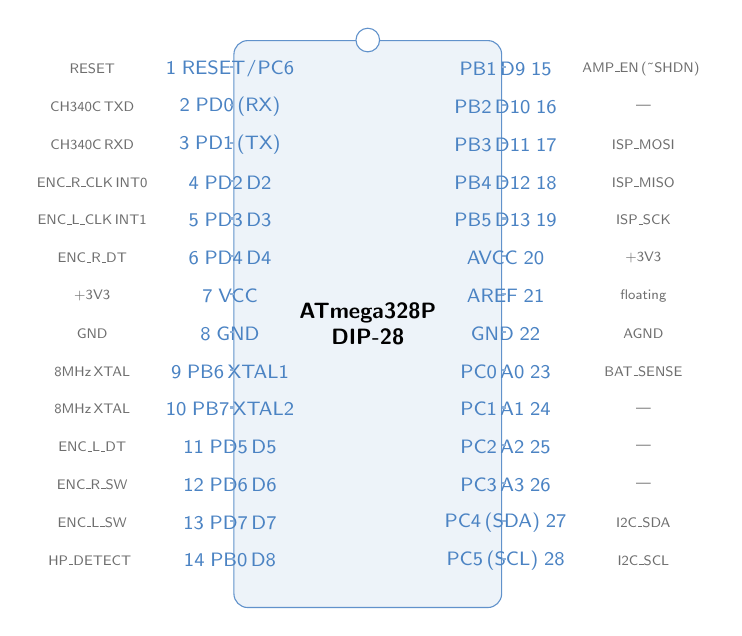
\begin{tikzpicture}[
  ic/.style={draw=accentblue!70, fill=accentblue!8,
             minimum width=3.4cm, minimum height=7.2cm,
             font=\sffamily\footnotesize\bfseries, align=center},
  pinl/.style={font=\sffamily\scriptsize, align=right, color=accentblue!80},
  pinr/.style={font=\sffamily\scriptsize, align=left, color=accentblue!80},
  netl/.style={font=\sffamily\tiny, align=right, color=codegray},
  netr/.style={font=\sffamily\tiny, align=left, color=codegray},
  wire/.style={thick, color=accentblue!50}
]
\node[ic, rounded corners=5pt] (mcu) {ATmega328P\\DIP-28};

% Left pins (1..14 top to bottom)
\pgfmathsetmacro{\pinspace}{7.2/15}
\foreach \n/\name/\net in {
  1/RESET$\slash$PC6/RESET,
  2/PD0\,(RX)/CH340C\,TXD,
  3/PD1\,(TX)/CH340C\,RXD,
  4/PD2\,D2/ENC\_R\_CLK\,INT0,
  5/PD3\,D3/ENC\_L\_CLK\,INT1,
  6/PD4\,D4/ENC\_R\_DT,
  7/VCC/{+3V3},
  8/GND/GND,
  9/PB6\,XTAL1/8MHz\,XTAL,
  10/PB7\,XTAL2/8MHz\,XTAL,
  11/PD5\,D5/ENC\_L\_DT,
  12/PD6\,D6/ENC\_R\_SW,
  13/PD7\,D7/ENC\_L\_SW,
  14/PB0\,D8/HP\_DETECT
} {
  \pgfmathsetmacro{\ypos}{3.24 - (\n-1)*\pinspace}
  \node[pinl] at (-1.75, \ypos) {\n\;\name};
  \node[netl] at (-3.5, \ypos) {\net};
  \draw[wire] (-1.75,\ypos+0.02) -- (-1.7,\ypos+0.02);
}

% Right pins (28..15 top to bottom)
\foreach \n/\name/\net in {
  28/PC5\,(SCL)/I2C\_SCL,
  27/PC4\,(SDA)/I2C\_SDA,
  26/PC3\,A3/{---},
  25/PC2\,A2/{---},
  24/PC1\,A1/{---},
  23/PC0\,A0/BAT\_SENSE,
  22/GND/AGND,
  21/AREF/{floating},
  20/AVCC/{+3V3},
  19/PB5\,D13/ISP\_SCK,
  18/PB4\,D12/ISP\_MISO,
  17/PB3\,D11/ISP\_MOSI,
  16/PB2\,D10/{---},
  15/PB1\,D9/AMP\_EN\,(\textasciitilde SHDN)
} {
  \pgfmathsetmacro{\idx}{\n-15}
  \pgfmathsetmacro{\ypos}{3.24 - \idx*\pinspace}
  \node[pinr] at (1.75, \ypos) {\name\;\n};
  \node[netr] at (3.5, \ypos) {\net};
  \draw[wire] (1.7,\ypos+0.02) -- (1.75,\ypos+0.02);
}

% Notch at top
\node[draw=accentblue!70, fill=white, circle, minimum size=0.3cm, inner sep=0pt]
  at (mcu.north) {};

\end{tikzpicture}
\end{diagrambox}

% ============================================================================
\section{RDA5807M Key Registers}
% ============================================================================

\begin{longtable}{@{}p{1.5cm}p{3cm}p{8cm}@{}}
\toprule
\textbf{Reg} & \textbf{Init Value} & \textbf{Key Bits} \\
\midrule
\endhead
0x02 & 0xC001 & [15] DHIZ=1 (audio high-Z disable), [14] DMUTE=1 (unmute), [0] ENABLE=1 \\
0x03 & (channel) & [15:6] CHAN (frequency channel), [4] TUNE (start tuning), [3:2] BAND=00 (87-108), [1:0] SPACE=00 (100kHz) \\
0x04 & 0x0A00 & [11] DE=1 (50\,$\mu$s de-emphasis), [9] SOFTMUTE\_EN=1 \\
0x05 & 0x88Ax & [15:12] INT\_MODE, [11:8] SEEKTH=8, [3:0] VOLUME (0--15) \\
0x0A & (read) & [14] STC (seek/tune complete), [13] SF (seek fail), [9:0] READCHAN \\
0x0B & (read) & [15:9] RSSI (signal strength, 0--127) \\
\bottomrule
\end{longtable}

Frequency formula: $\text{Channel} = \frac{\text{Freq(MHz)} - 87.0}{0.1}$ \quad (Band=00, Space=00)

Reverse: $\text{Freq(MHz)} = 87.0 + \text{Channel} \times 0.1$

% ============================================================================
\section{KiCad Custom Library Quick Reference}
% ============================================================================

Components you must import or create (not in KiCad default libraries):

\begin{longtable}{@{}p{3.5cm}p{3cm}p{6cm}@{}}
\toprule
\textbf{Component} & \textbf{Source} & \textbf{Import Method} \\
\midrule
\endhead
PAM8403 (SOP-16) & SnapEDA & SnapEDA download; footprint \texttt{Package\_SO:SOP-16\_4.4x10.4mm\_P1.27mm} \\
CH340C (SOP-16) & SnapEDA or LCSC & SnapEDA download; footprint \texttt{Package\_SO:SOP-16\_4.4x10.4mm\_P1.27mm} \\
TP4056 (SOP-8) & SnapEDA & SnapEDA download; footprint \texttt{Package\_SO:SOP-8\_3.9x4.9mm\_P1.27mm} \\
HT7333 (SOT-89) & SnapEDA & SnapEDA download; footprint \texttt{Package\_TO\_SOT\_SMD:SOT-89-3} \\
DW01A (SOT-23) & SnapEDA & SnapEDA download; footprint \texttt{Package\_TO\_SOT\_SMD:SOT-23} \\
FS8205A (SOT-23-6) & SnapEDA & SnapEDA download; footprint \texttt{Package\_TO\_SOT\_SMD:SOT-23-6} \\
USB-C receptacle & SnapEDA or LCSC & Depends on exact part; 16-pin SMD footprint \\
RRD-102 V2.0 module & Create manually & Custom symbol (10 pins) + custom footprint (11$\times$11mm, 1.27mm pitch) \\
SSD1306 OLED module & Create manually & Simple 4-pin symbol + use built-in 1$\times$4 header footprint \\
3.5mm Audio Jack & KiCad built-in & \texttt{Connector\_Audio:AudioJack3\_SwitchT} \\
Rotary Encoder & KiCad built-in & \texttt{Device:RotaryEncoder\_Switch} \\
ATmega328P-PU & KiCad built-in & \texttt{MCU\_Microchip\_ATmega:ATmega328P-PU} \\
Crystal & KiCad built-in & \texttt{Device:Crystal} \\
\bottomrule
\end{longtable}

\vfill
\begin{center}
\rule{0.5\textwidth}{0.5pt}\\[0.5cm]
\textit{End of document. Good luck with your pocket radio!}
\end{center}

\end{document}
